\documentclass{scrartcl}
\usepackage{graphicx}
\usepackage{amsmath}
\usepackage{listings}
\usepackage{mathtools}
\usepackage{physics}
\usepackage{siunitx}
\usepackage{tikz}
\usepackage{mathtools}
\usepackage{rotating}
\usepackage{hyperref}
\usepackage{fancyhdr}

\pagestyle{fancy}
\fancyhf{}
\rhead{Jamie Grieser}
\lhead{Simulation Methods}
\rfoot{Page \thepage}

\definecolor{mygreen}{rgb}{0,0.6,0}
\definecolor{mygray}{rgb}{0.5,0.5,0.5}
\definecolor{mymauve}{rgb}{0.58,0,0.82}

\lstset{ 
	backgroundcolor=\color{white},   % choose the background color; you must add \usepackage{color} or \usepackage{xcolor}; should come as last argument
	basicstyle=\footnotesize,        % the size of the fonts that are used for the code
	breakatwhitespace=false,         % sets if automatic breaks should only happen at whitespace
	breaklines=true,                 % sets automatic line breaking
	captionpos=b,                    % sets the caption-position to bottom
	commentstyle=\color{mygreen},    % comment style
	deletekeywords={...},            % if you want to delete keywords from the given language
	escapeinside={\%*}{*)},          % if you want to add LaTeX within your code
	extendedchars=true,              % lets you use non-ASCII characters; for 8-bits encodings only, does not work with UTF-8
	frame=single,	                   % adds a frame around the code
	keepspaces=false,                 % keeps spaces in text, useful for keeping indentation of code (possibly needs columns=flexible)
	keywordstyle=\color{blue},       % keyword style
	language=Octave,                 % the language of the code
	morekeywords={*,...},            % if you want to add more keywords to the set
	numbers=left,                    % where to put the line-numbers; possible values are (none, left, right)
	numbersep=5pt,                   % how far the line-numbers are from the code
	numberstyle=\tiny\color{mygray}, % the style that is used for the line-numbers
	rulecolor=\color{black},         % if not set, the frame-color may be changed on line-breaks within not-black text (e.g. comments (green here))
	%showspaces=false,                % show spaces everywhere adding particular underscores; it overrides 'showstringspaces'
	showstringspaces=false,          % underline spaces within strings only
	showtabs=false,                  % show tabs within strings adding particular underscores
	stepnumber=2,                    % the step between two line-numbers. If it's 1, each line will be numbered
	stringstyle=\color{mymauve},     % string literal style
	tabsize=2,	                   % sets default tabsize to 2 spaces
	%title=\lstname                   % show the filename of files included with \lstinputlisting; also try caption instead of title
}

\begin{document}

\section*{Problem Sheet 5}
\subsection*{Exercise 1.1}

Comment of the author:\\
When programming this exercise, I realized, that it is much easier to consider a \( 30 \times 30 \) grid reaching from 0 to \(2H\) because this is much simpler to represent in Python.

Before we can start the exercise, we have to devise a scheme to determine the cell where the particle with position \( (X_i, Y_i) \) can be found. To do this, we use the relations
\begin{align}
	x_k = k + \frac{H}{K} \\
	y_l = l + \frac{H}{K} 
\end{align}
for the position of the center \( (x_k, y_l) \) of the cell \( (k,l) \). We can reshape these relations and use the floor() function to obtain the cell indices.
\begin{align}
	k = \Big \lfloor X_i - \frac{H}{K} \Big \rfloor \\
	l = \Big \lfloor Y_i - \frac{H}{K} \Big \rfloor
\end{align}
This can be simplified further by assuming that the cell is enumerated by the lower left vertex of the cell, i.e. \( (15.3, 4.9) \) is in the cell with the position \( (15, 4) \). In that case, we can drop the \( \frac{H}{K} \)-part and write
\begin{align}
k = \Big \lfloor X_i \Big \rfloor \\
l = \Big \lfloor Y_i \Big \rfloor
\end{align}
Or as python code:
\begin{lstlisting}[title=Function to calculate the index., language=Python, frame=single]
def indices(X, Y):
	k = np.floor(X)
	j = np.floor(Y)
	return [int(k), int(j)]
\end{lstlisting}
Now that we know the cells where our particles are located, we obtain the numerical form of \( \rho(x,y) \) by calculating
\begin{equation}
	\rho_{kl} = \sum_{i=1}^N W_{kl}(X_i, Y_i)
\end{equation}
where the weight functions are given through
\begin{align}\label{weights}
	W_{kl}(x,y) & = \iint dx dy \Pi\Big(\frac{x-x_k}{2H/K}\Big)\Pi\Big(\frac{y-y_k}{2H/K}\Big)
					\delta(x-x_i)\delta(y-y_i)\\
				& = \Pi\Big(\frac{x_i-x_k}{2H/K}\Big)\Pi\Big(\frac{y_i-y_k}{2H/K}\Big)
\end{align}
This function is equal to 1 only when the particle is in th respective cell and 0 elsewhere.
\subsection*{Exercise 1.2}
In the generalization to a \( 3 \times 3 \)-stencil, we can simply write the \(0^{th}\) order as 
\begin{equation}
	\text{w}[:,:] = \begin{pmatrix}
	0 & 0 & 0 \\
	0 & 1 & 0 \\
	0 & 0 & 0
	\end{pmatrix}.
\end{equation}
Before we continue with the derivation for the \( 1^{st} \)- and \( 2^{nd} \)-order stencil, we introduce the following notation to make the derivation easier:
\begin{equation}
	\epsilon_x = \dfrac{X_i - x_{k-1/2}}{x_{k+1/2} - x_{k-1/2}}
\end{equation}

\subsection*{Exercise 1.2}

and the same for \( \epsilon_y \) in the y-direction. 
We will assume a cell length of 1 to increase readability. The following sketch \ref{fig:sketch01} shows the geometric interpretation of this.
\begin{figure}[h]
	\centering
	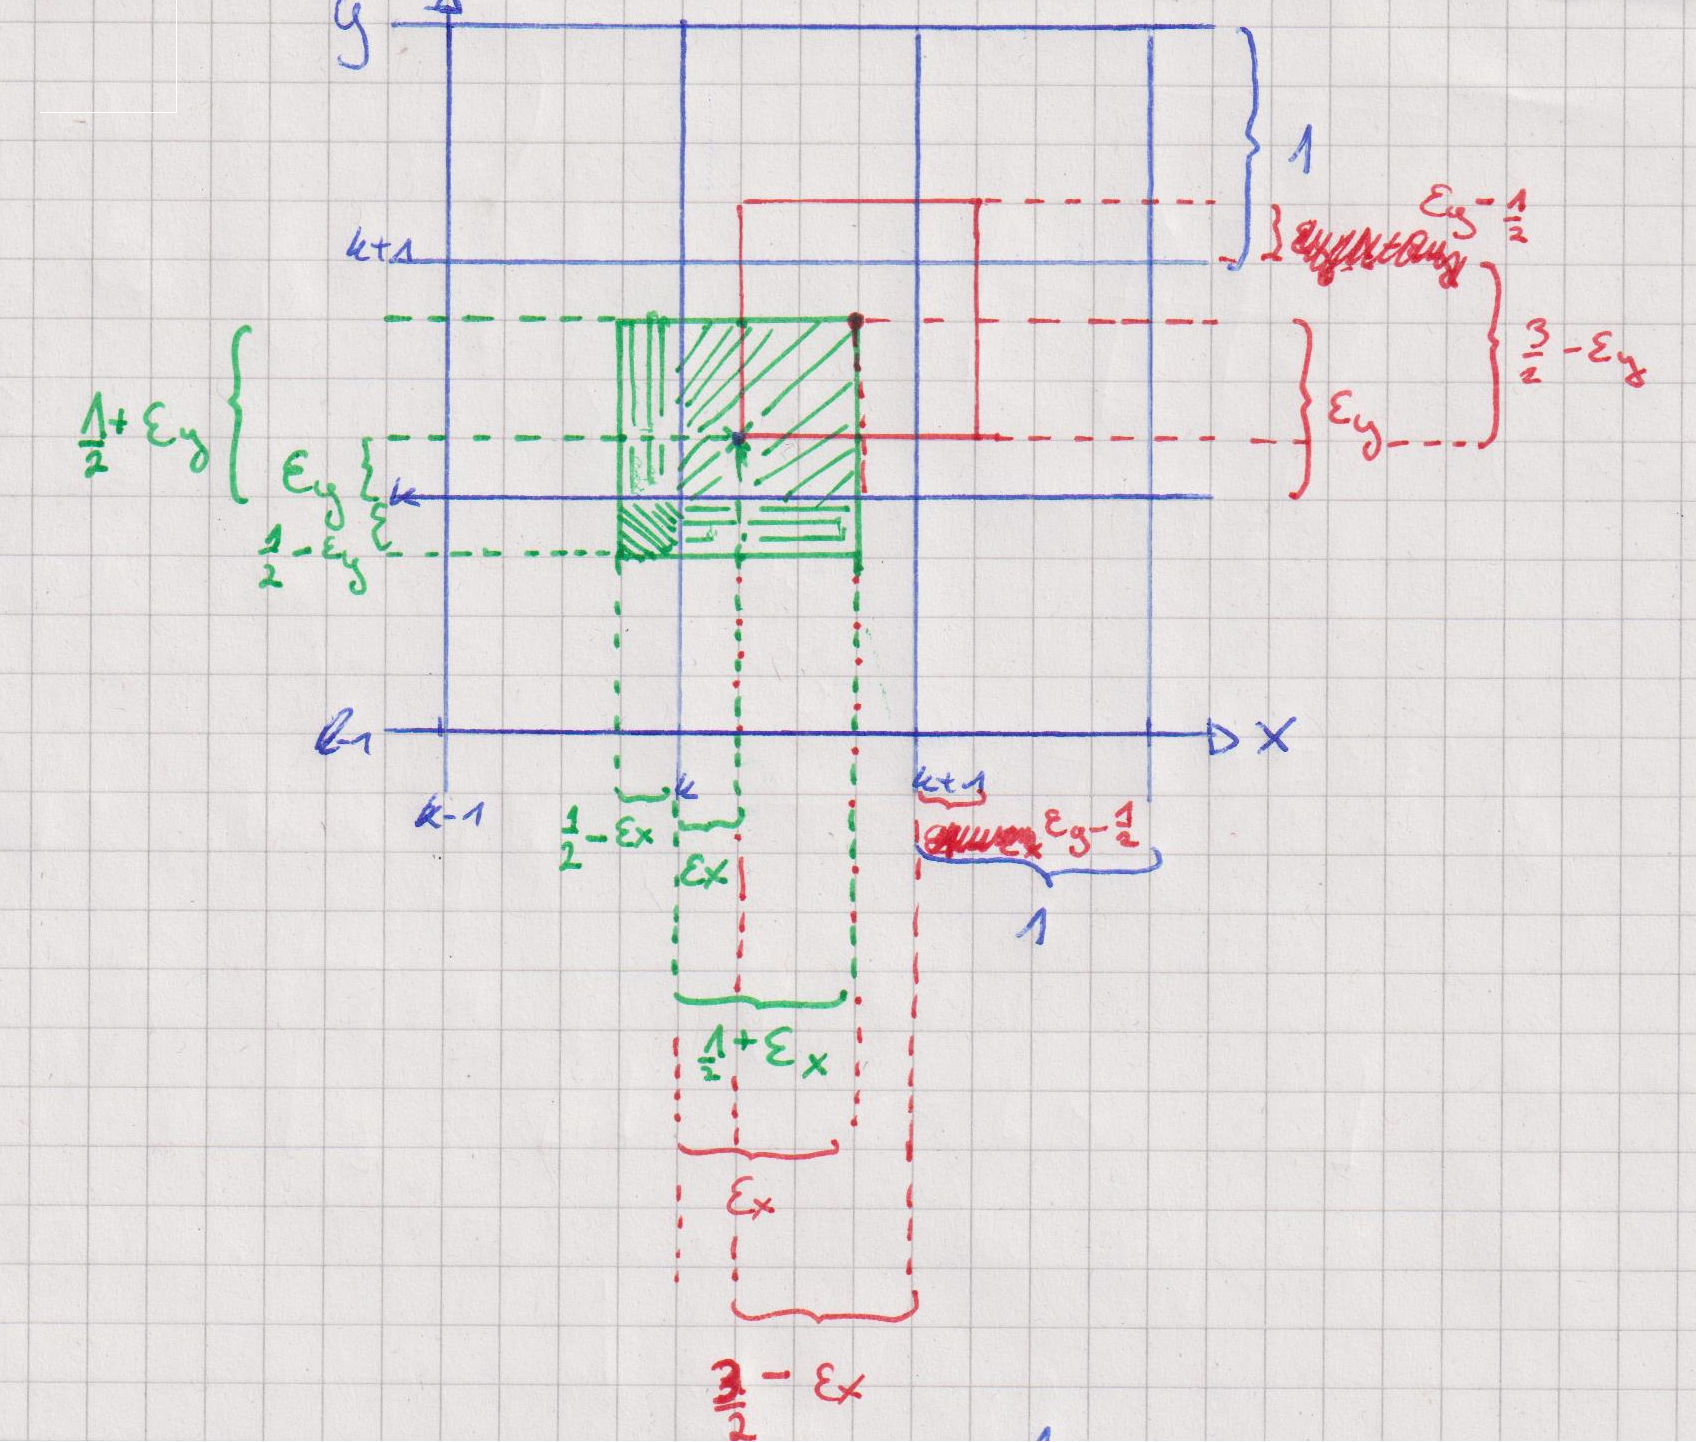
\includegraphics[width=0.7\linewidth]{Plots/sketch01}
	\caption{Geometric interpretation for the devised algortihm. The green triangle satisfies \( \epsilon_x, \epsilon_y < \frac{1}{2} \), while the red triangle satisfies \( \epsilon_x, \epsilon_y > \frac{1}{2} \). Depending on the size of the epsilons, different cells are filled. We also see that the formulas for the areas in the squares depend on the epsilons. The height of the cubucle is one and thus ignored.}
	\label{fig:sketch01}
\end{figure}
We now begin with the \( 1^{st} \)-order derivation. To do this, we replace the \(\delta\)-distribution of the 0-th order by a top-hat function. Thus the integral in \eqref{weights} gives as a result the overlap between cloud cubicle of the particle and the adjacent cells. 
The overlap can be simply expressed in terms of \( \epsilon_x \) and \( \epsilon_y \). We immediately see that the cloud can overlap with 4 cells at most. The overlap for all four non-zero weights in the sketch reads:
\begin{align*}
	&W_{k,l} = \Big(\frac{1}{2} + \epsilon_x\Big) \Big(\frac{1}{2} + \epsilon_y\Big)\\
	&W_{k-,l-1} = \epsilon_x \epsilon_y\\
	&W_{k,l-1} = \Big(\frac{1}{2} + \epsilon_x\Big) \Big(\frac{1}{2} - \epsilon_y\Big)\\
	&W_{k-1,l} = \Big(\frac{1}{2}-\epsilon_x\Big) \Big(\frac{1}{2} + \epsilon_y\Big)
\end{align*}
All other weights are zero.
The weights satisfy the normalization condition for their sum to be equal to unity. This works of course only if \( \epsilon_x, \epsilon_y < \frac{1}{2}\). For the case of one or both of them being bigger, we have to replace some of the weights. To see how this is done, consider figure ().
This algorithm is implemented in the following way:
\begin{lstlisting}[title=Function to calculate the 1st order., language=Python, frame=single]
def compute_1_order(X, Y, k, l):
	W = np.ones((3, 3))
	ex = calculate_e(X, k)
	ey = calculate_e(Y, l)
	if ex < 0.5:
		W[:, 0] *= H/K - ex
		W[:, 1] *= ex + H/K
		W[:, 2] *= 0
	else:
		W[:, 0] *= 0
		W[:, 1] *= 3*H/K - ex
		W[:, 2] *= ex - H/K
	
	if ey < 0.5:
		W[0, :] *= H/K - ey
		W[1, :] *= ey + H/K
		W[2, :] *= 0
	else:
		W[0, :] *= 0
		W[1, :] *= 3*H/K - ey
		W[2, :] *= ey - H/K
	return W
\end{lstlisting}
In a similar manner, we can derive the solution for the \( 2^{nd} \)-order algorithm. First, we realize, that we no longer have a cubical cloud shape with base 1 but instead a regular pyramid with baseline 2 and height 1. Thus, when calculating the volume of the cloud contained in a specific cell we have to take this into account. \\The following sketch \ref{fig:sketch02} shows again how to derive the weight matrix for the \( 2^{nd} \)-order method.
\begin{figure}[h]
	\centering
	\includegraphics[width=0.7\linewidth]{Plots/sketch02}
	\caption{Geometric interpretation for the second-order method. This time, the height depends on the epsilons. and we have to add an factor of \( \frac{1}{2} \) when calculating the area projected into the x or y-direction due to the triangular shape.}
	\label{fig:sketch02}
\end{figure}
We simply project the x and the y-part of the pyramid into a 2D plane. There we find the area, that contributes to the respective square to be width times height or length times height. \\To get the volume contained in the stencil cell, we multiply these two areas. For example, we multiply all cells in the row with index \( k-1 \) with the value 
\( \frac{(1-\epsilon_x)^2}{2} = \frac{1}{2} - \epsilon_x + \frac{\epsilon_x^2}{2}\) and their respectiv y-direction contribution.
From this, we can write an algorithm that calculates the stencil using:
\begin{lstlisting}[title=Function to calculate the 2nd order., language=Python, frame=single]
def compute_2_order(X, Y, k, l):
	ex = calculate_e(X, k)
	ey = calculate_e(Y, l)
	W = np.ones((3, 3))
	W[:, 0] *= 0.5 - ex + 0.5*ex**2
	W[:, 1] *= 0.5 + ex - ex ** 2
	W[:, 2] *= 0.5 * ex**2
	W[0, :] *= 0.5 - ey + 0.5 * ey ** 2
	W[1, :] *= 0.5 + ey - ey ** 2
	W[2, :] *= 0.5 * ey ** 2
	return W
\end{lstlisting}

\subsection*{Exercise 1.3}

After we obtained functions for the different methods, we use the \textit{density\_map()} function to calculate the density map:
\begin{lstlisting}[title=Function to calculate the 2nd order., language=Python, frame=single]
def density_map(particle_list, order):
	d_map = np.zeros((K, K))
		for k in range(1, K-1):
			for j in range(1, K-1):
				for particle in particle_list:
				x, y = particle[0], particle[1]  # particle position
				if indices(x, y) == [k, j]:
					W = compute_order(x, y, k, j, order)
					d_map[np.ix_([j-1, j, j+1], [k-1, k, k+1])] += M/N * W
	return d_map
\end{lstlisting}
This gives a Numpy array that contains the density map. To check whether everything is centered and calculated accordingly, we check some plots for the different functions in \ref{fig:0thorder}, \ref{fig:1storder} and \ref{fig:2ndorder}.
We see that the particles are placed accordingly.
\begin{figure}[h]
	\centering
	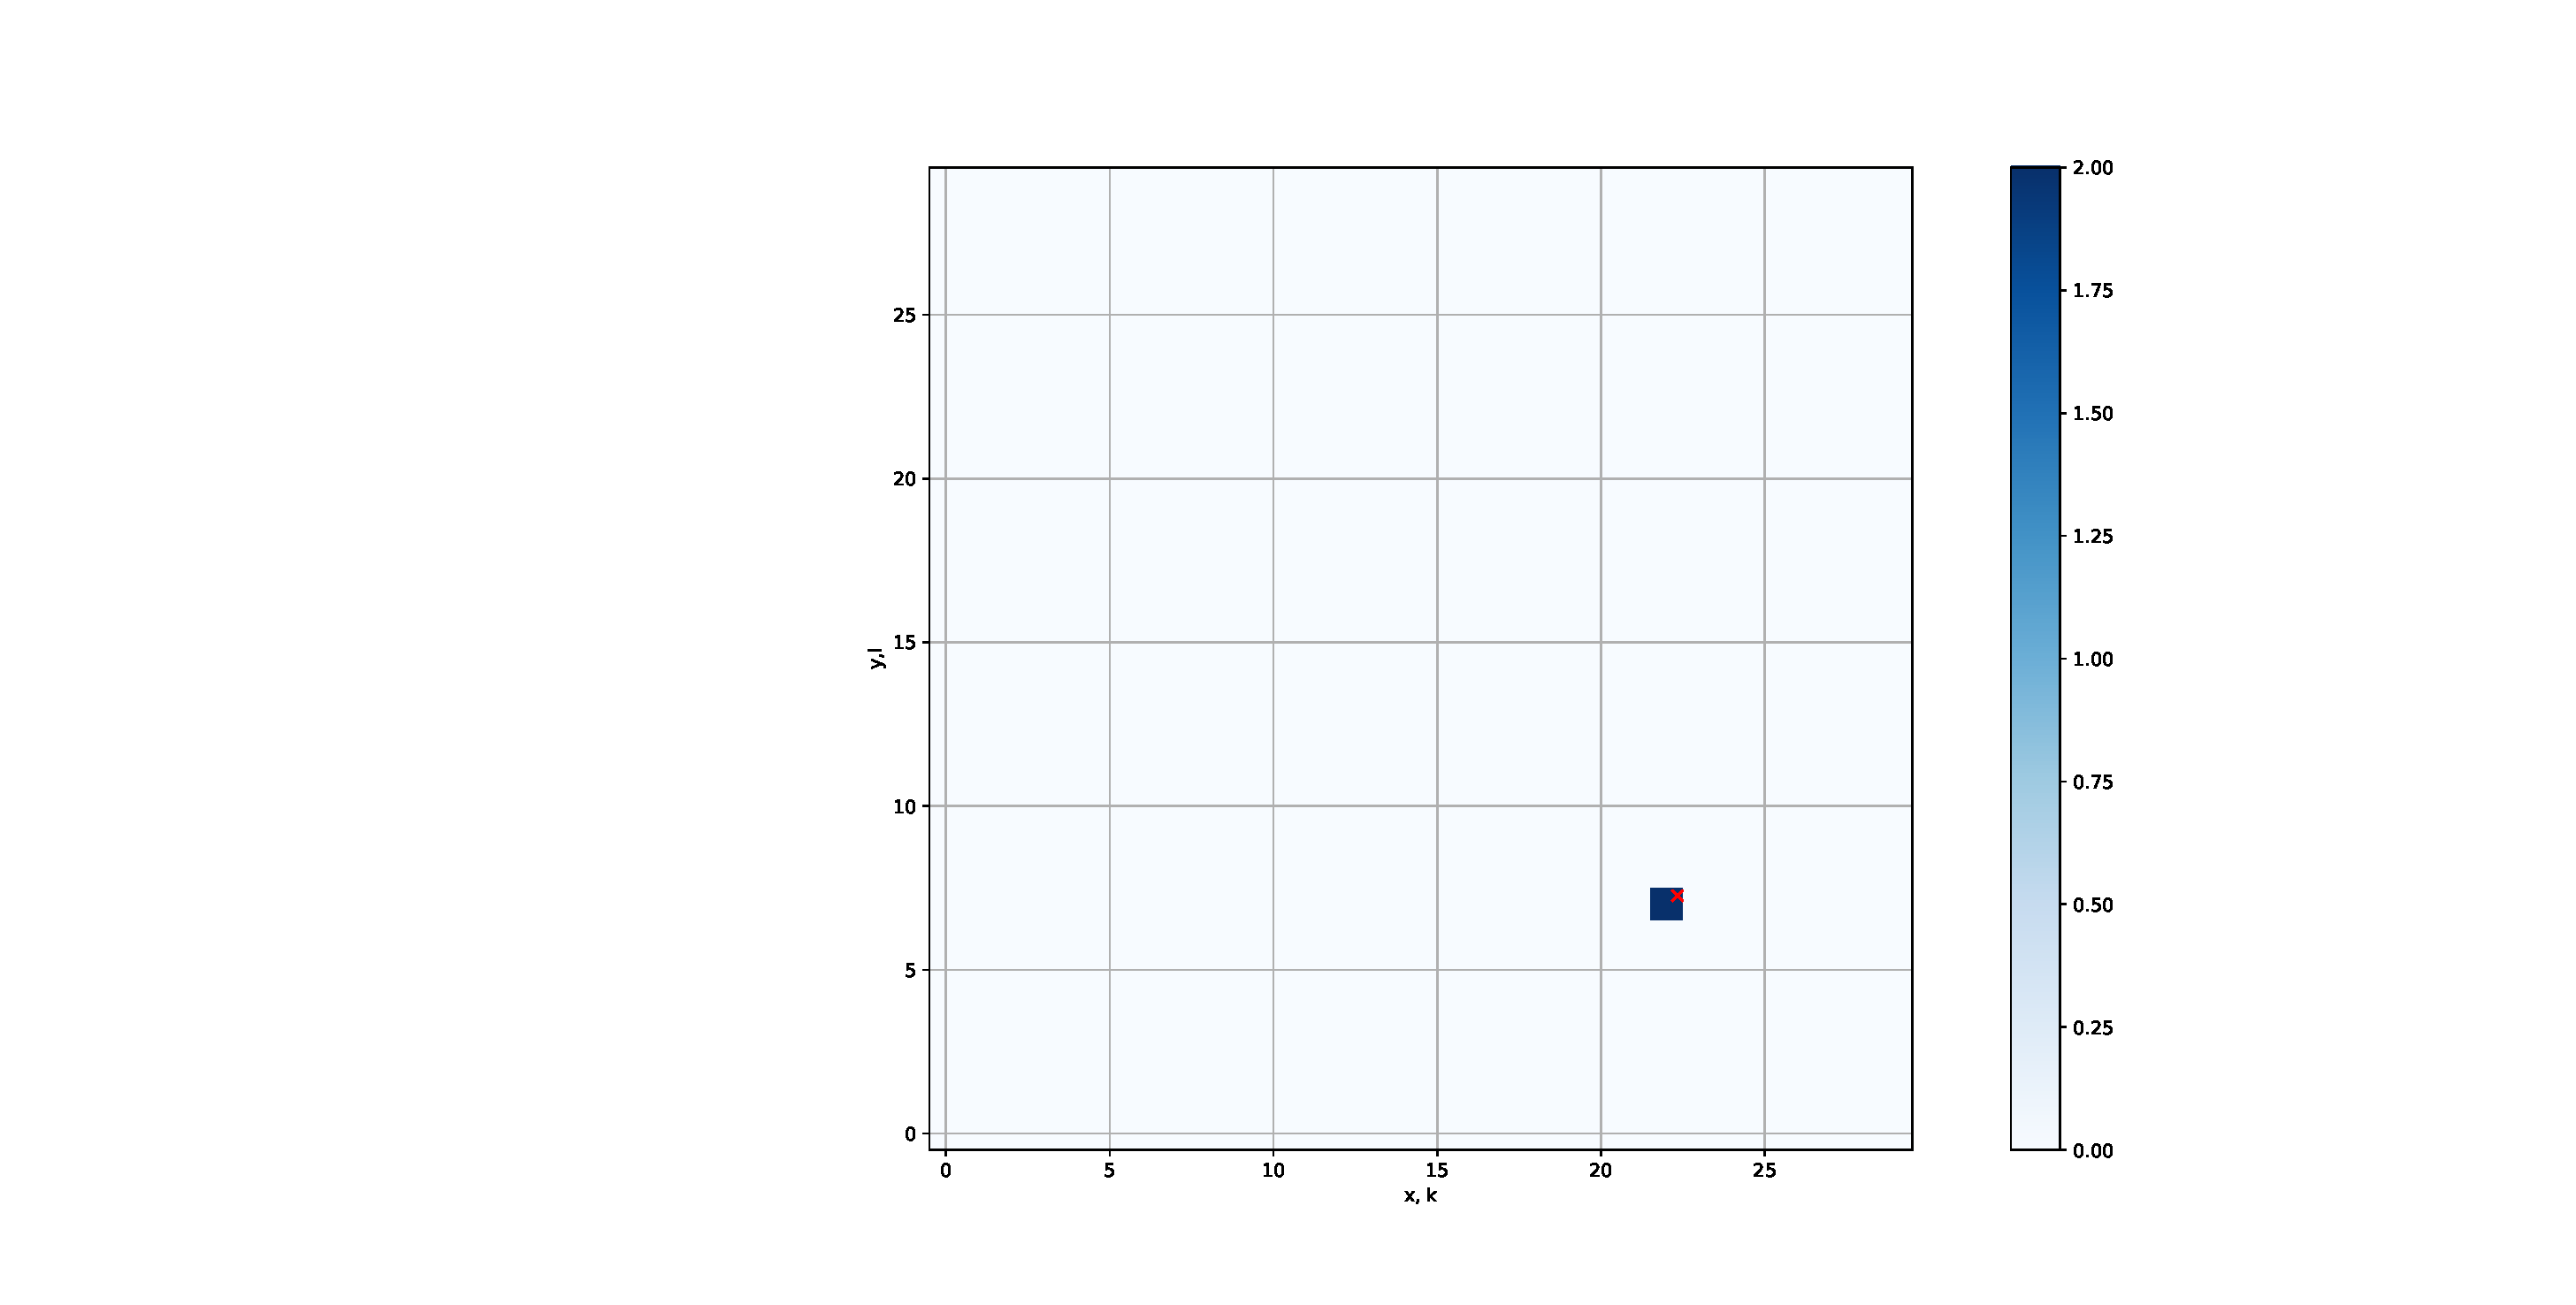
\includegraphics[width=0.9\linewidth]{Plots/0th_order.eps}
	\caption{One particle on the grid with the \(0^{th}\)-order method.}
	\label{fig:0thorder}
\end{figure}
\begin{figure}[h]
	\centering
	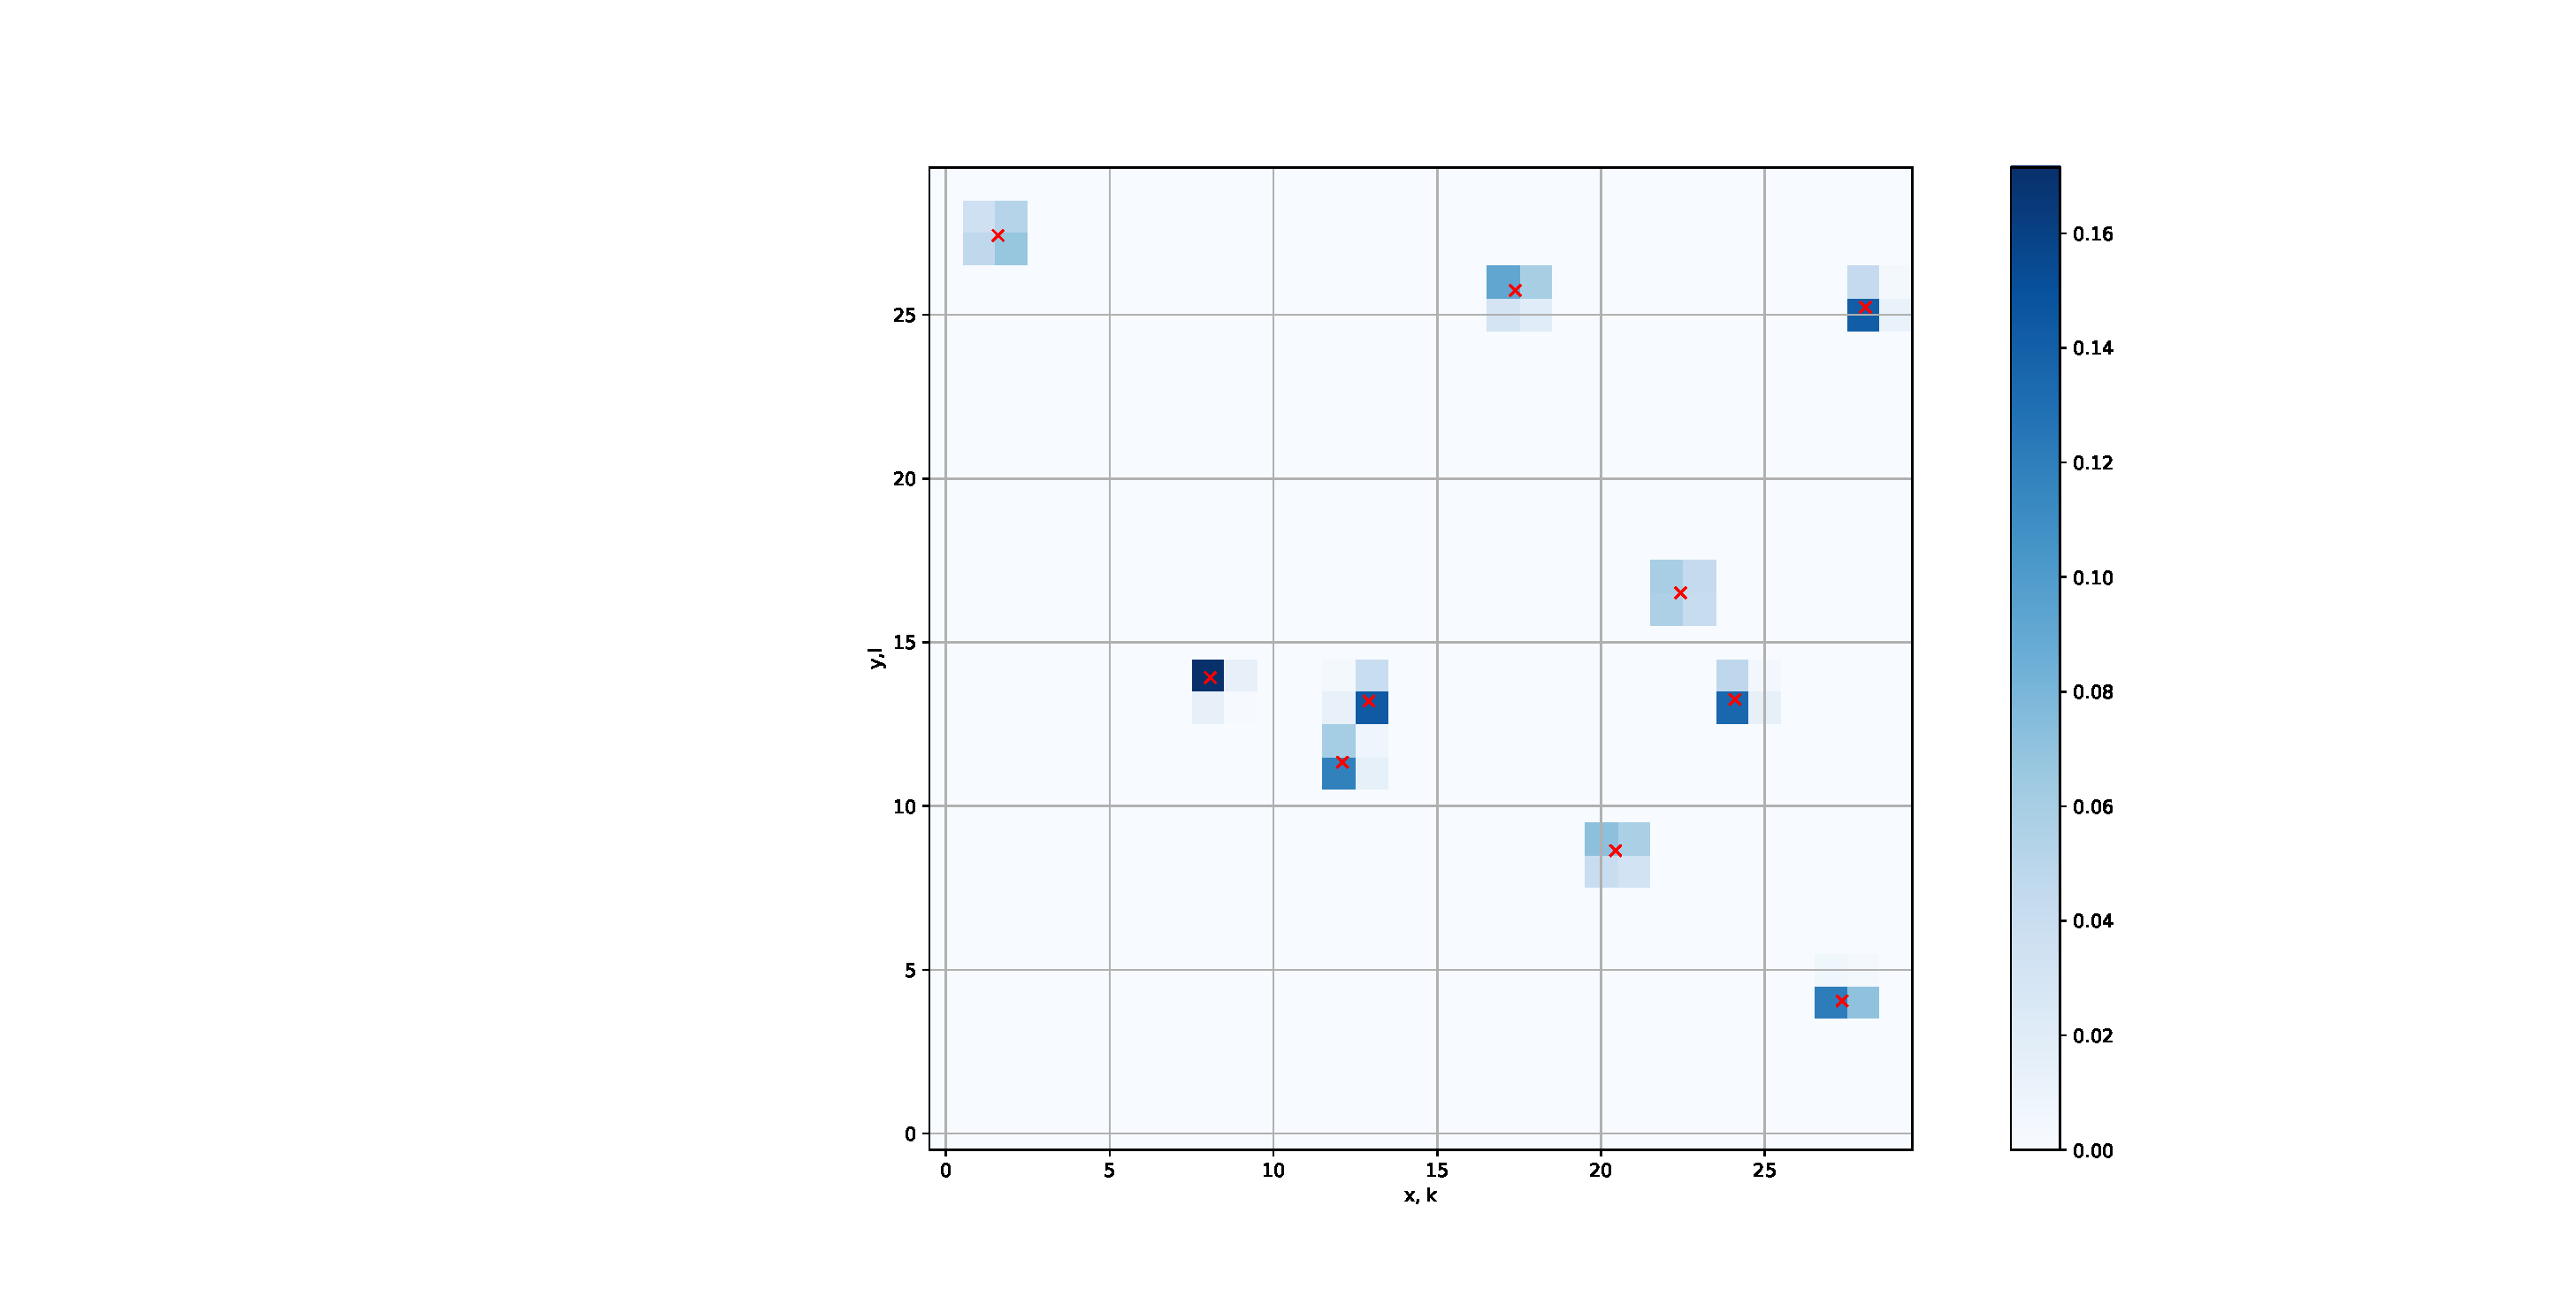
\includegraphics[width=0.9\linewidth]{Plots/1st_order.eps}
	\caption{Ten particles on the grid with the \(1^{st}\)-order method.}
	\label{fig:1storder}
\end{figure}
\begin{figure}[h]
	\centering
	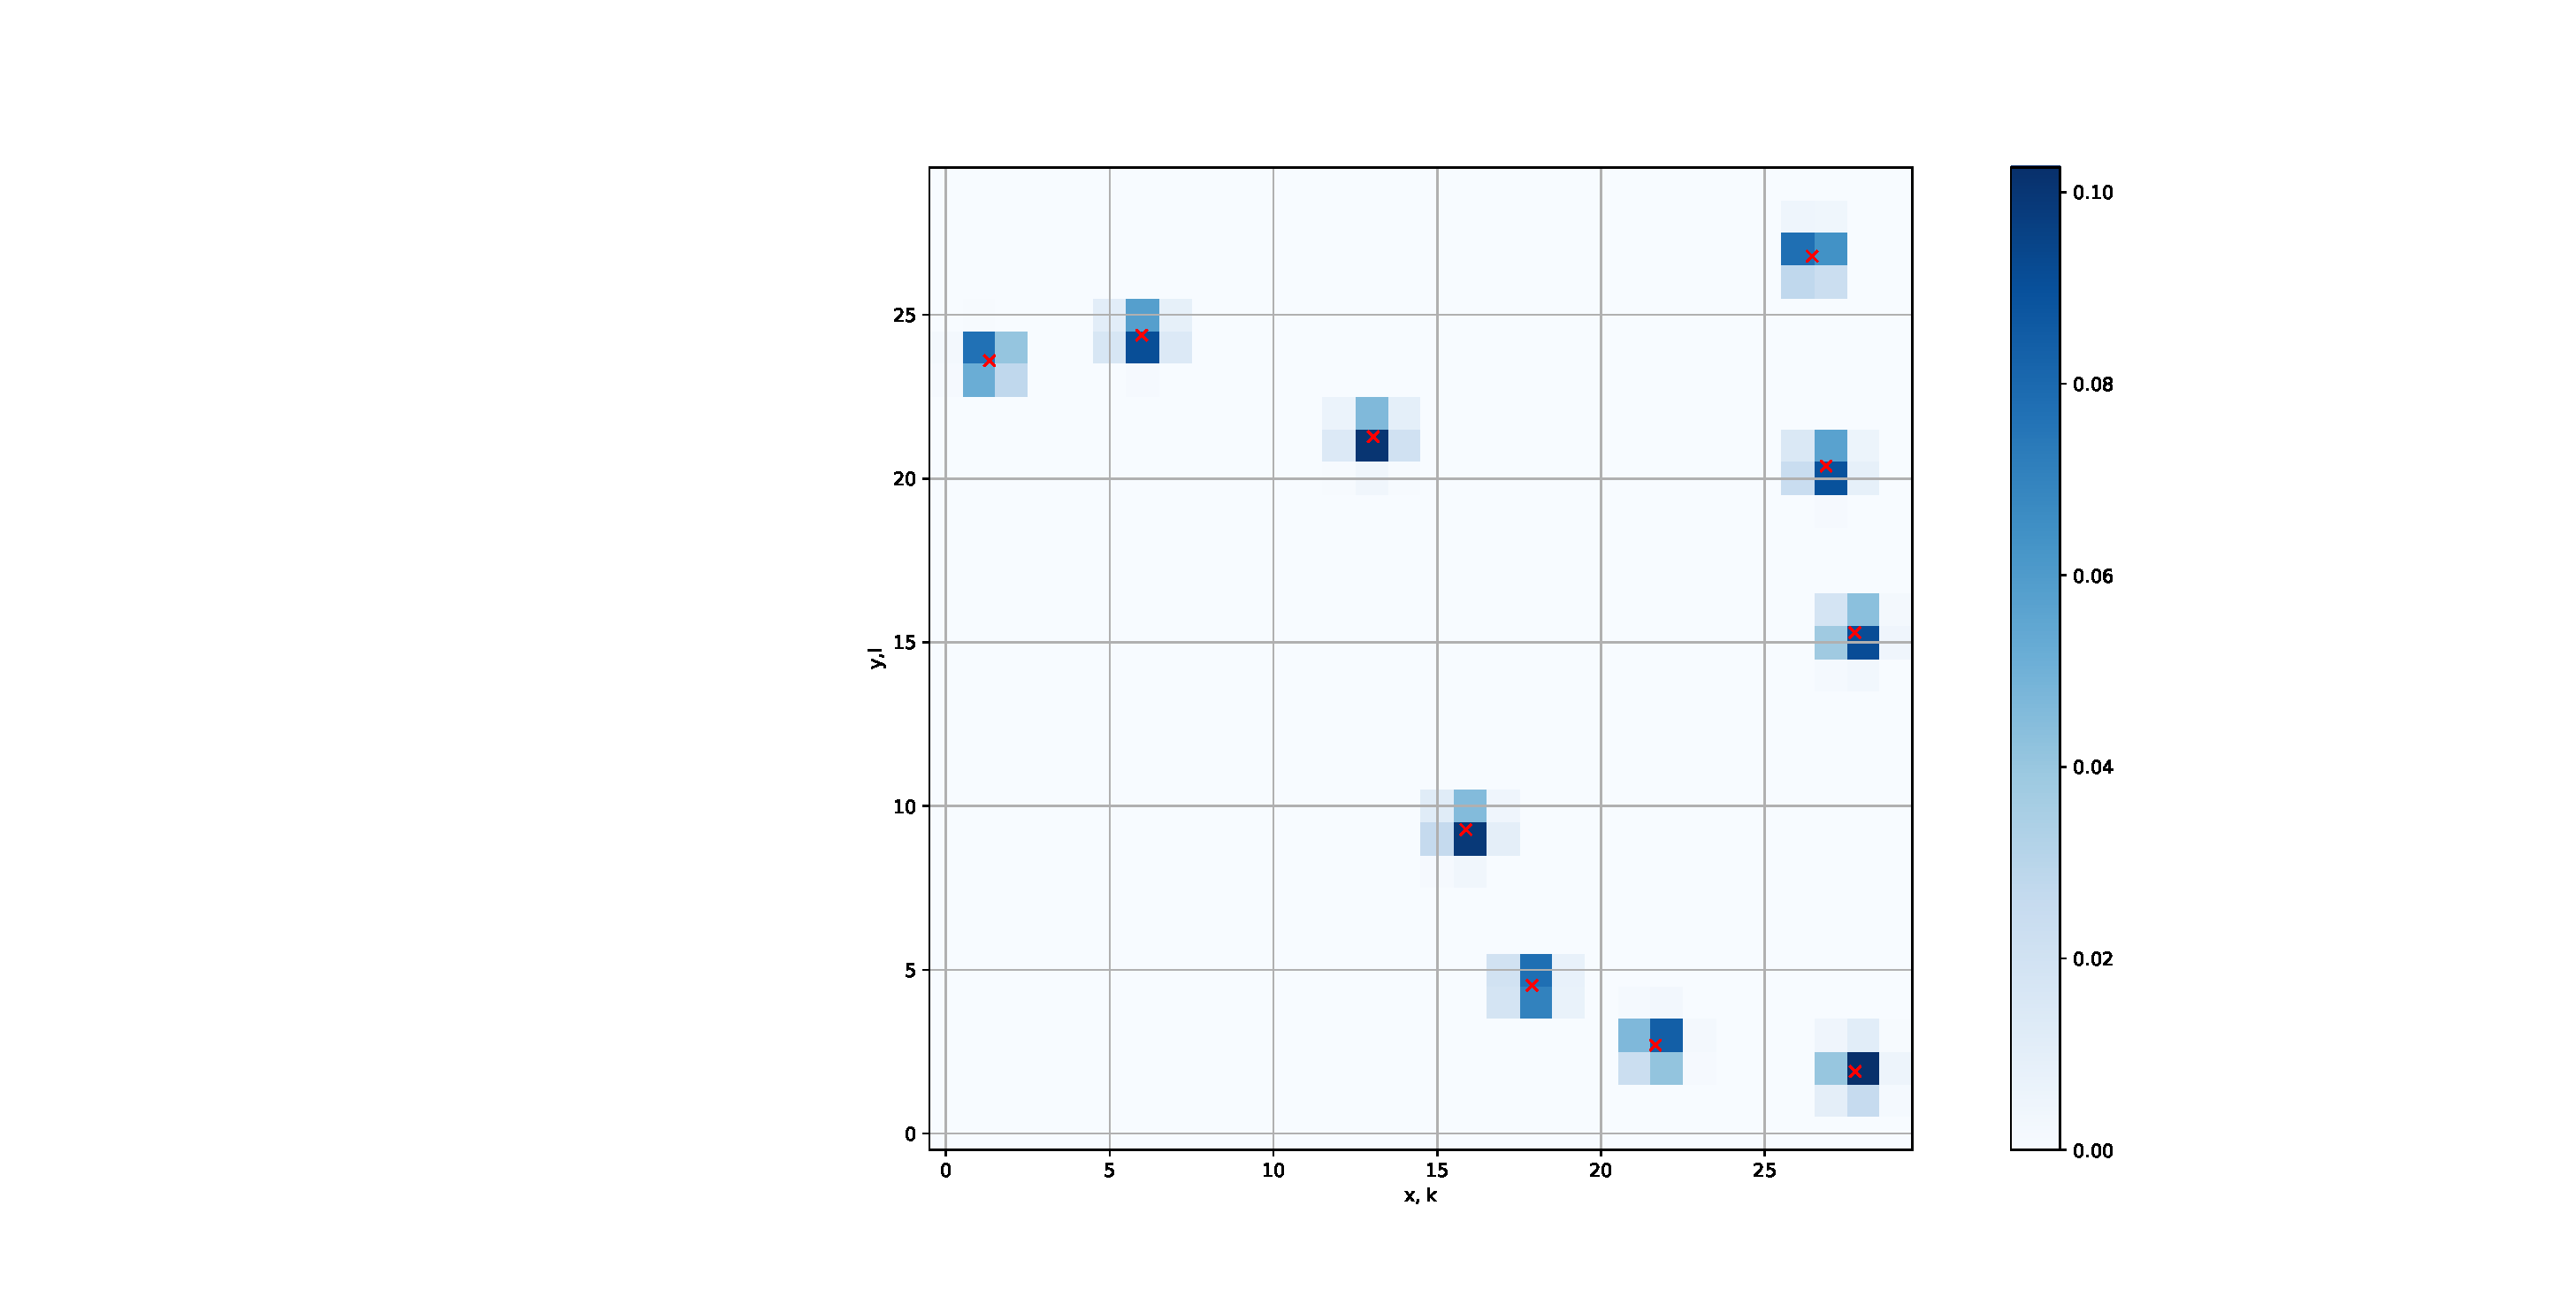
\includegraphics[width=0.9\linewidth]{Plots/2nd_order.eps}
	\caption{Ten particles on the grid with the \(2^{nd}\)-order method.}
	\label{fig:2ndorder}
\end{figure}

Next, we plot the same Gaussian distribution of 100 particles on the grid for different methods(see figures \ref{fig:n1000}, \ref{fig:n100001} and \ref{fig:n100002}). We immediately see the softening, that occurs when using higher orders.
\begin{figure}[h]
	\centering
	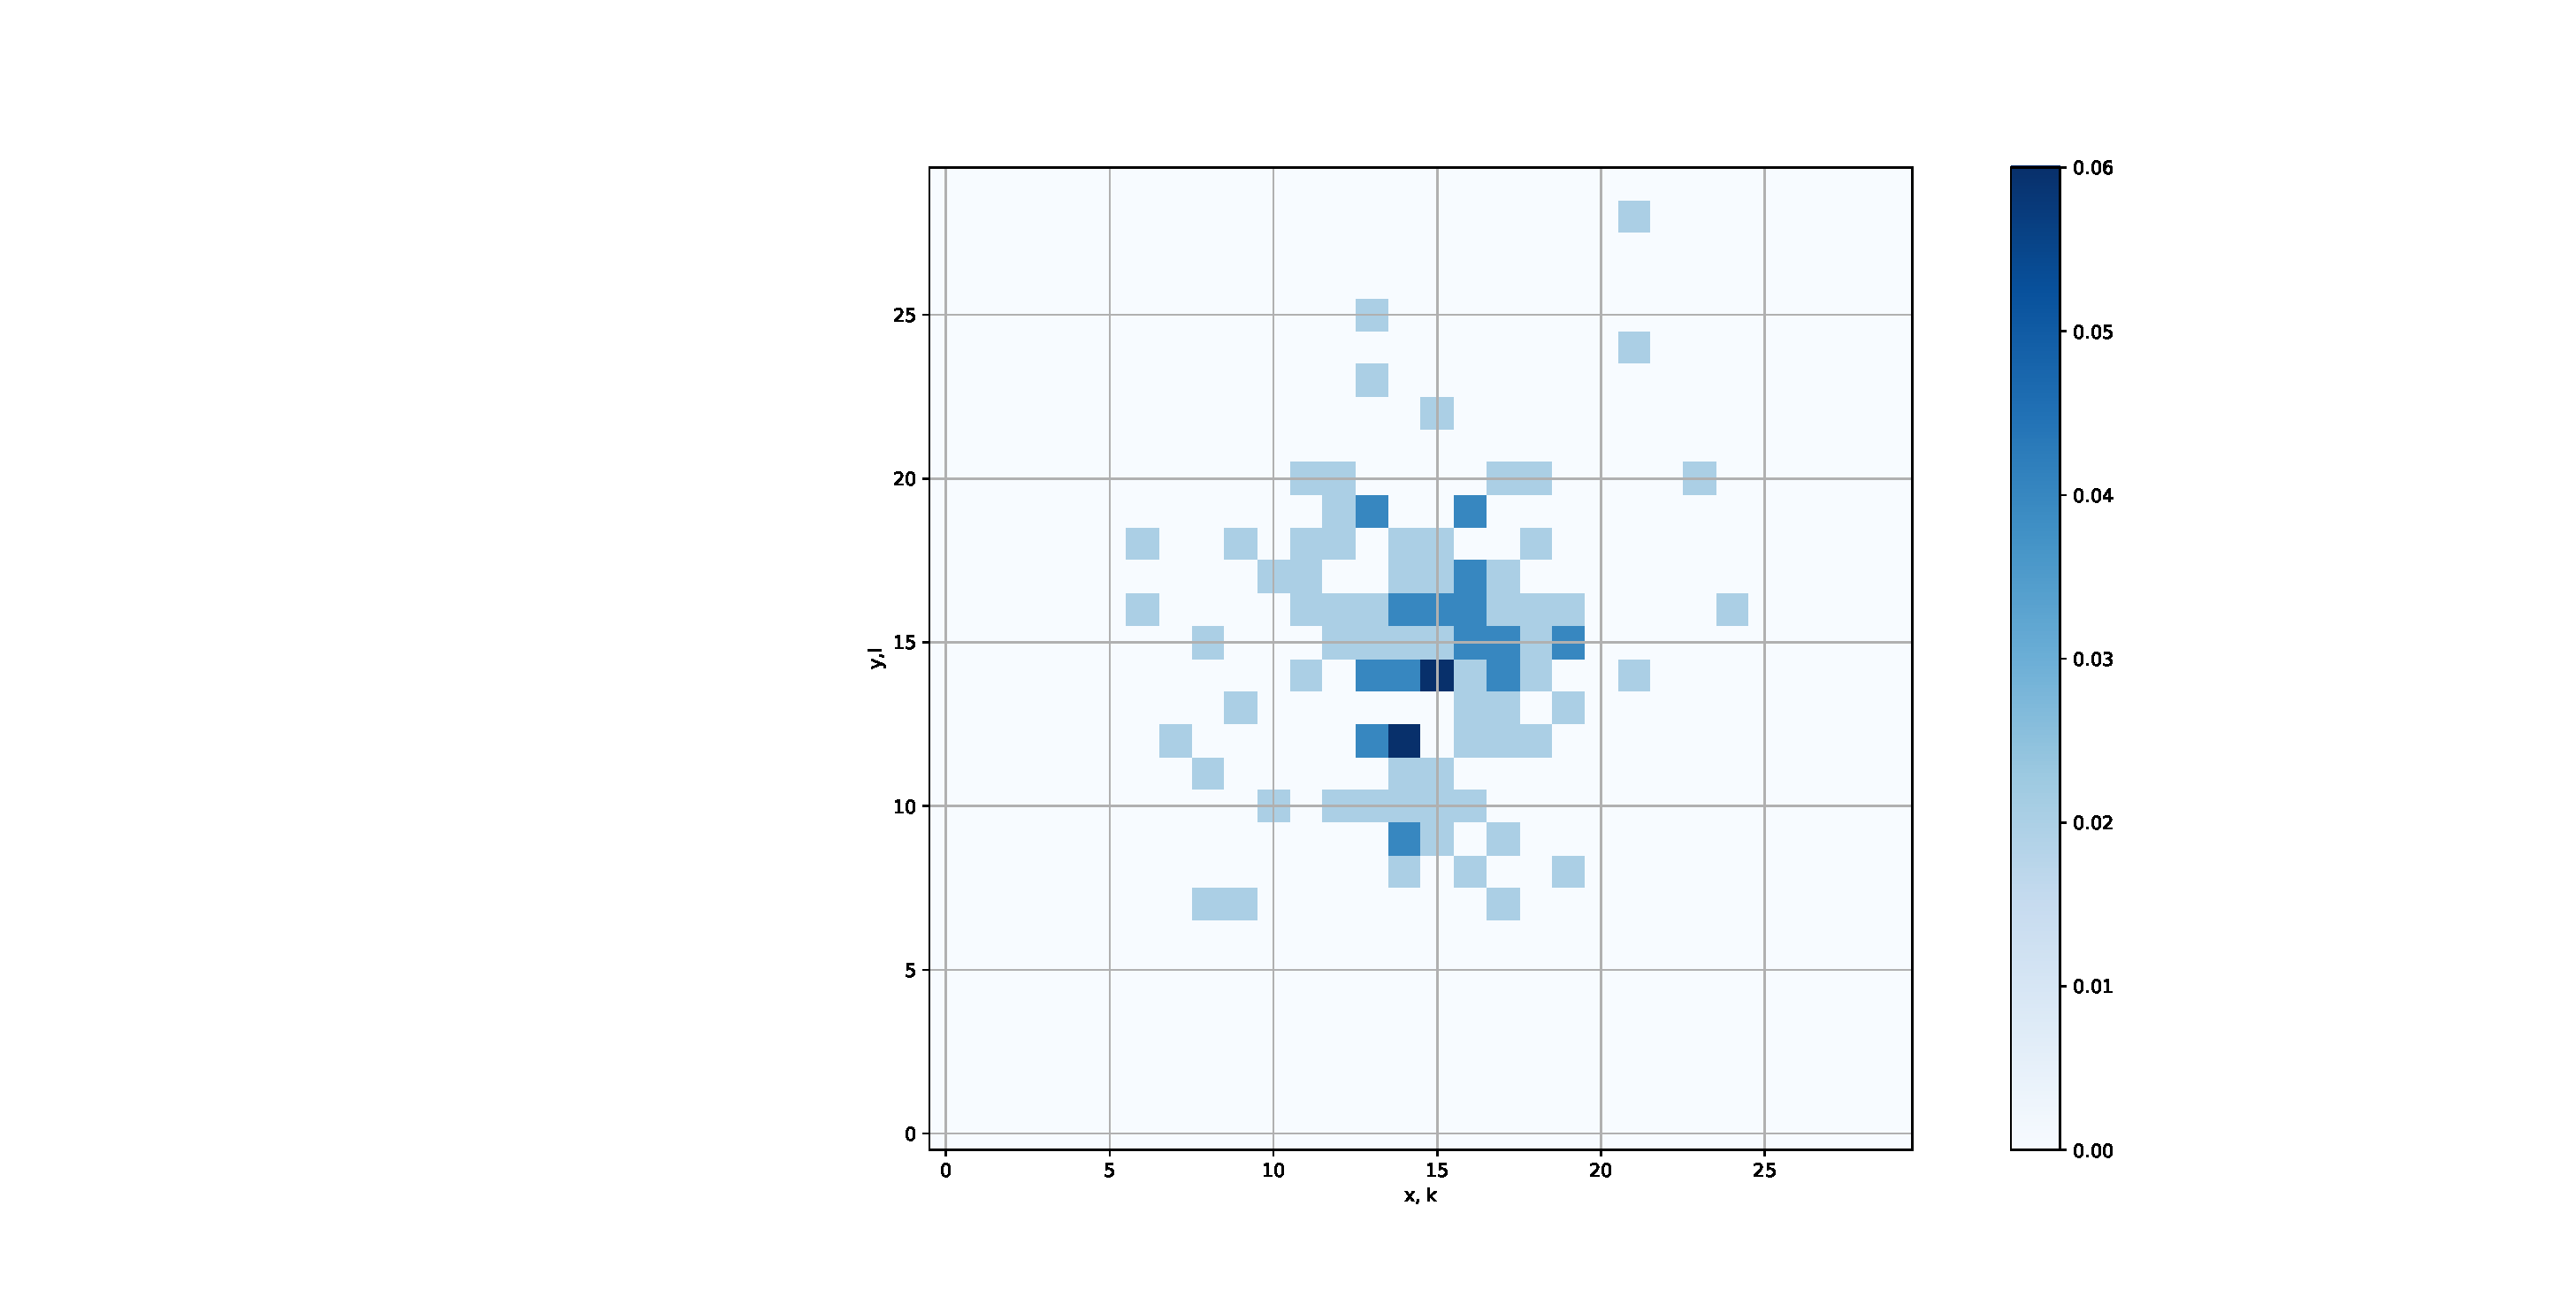
\includegraphics[width=0.9\linewidth]{Plots/N100_0}
	\caption{100 particles on the grid with the \(0^{th}\)-order method.}
	\label{fig:n1000}
\end{figure}
\begin{figure}[h]
	\centering
	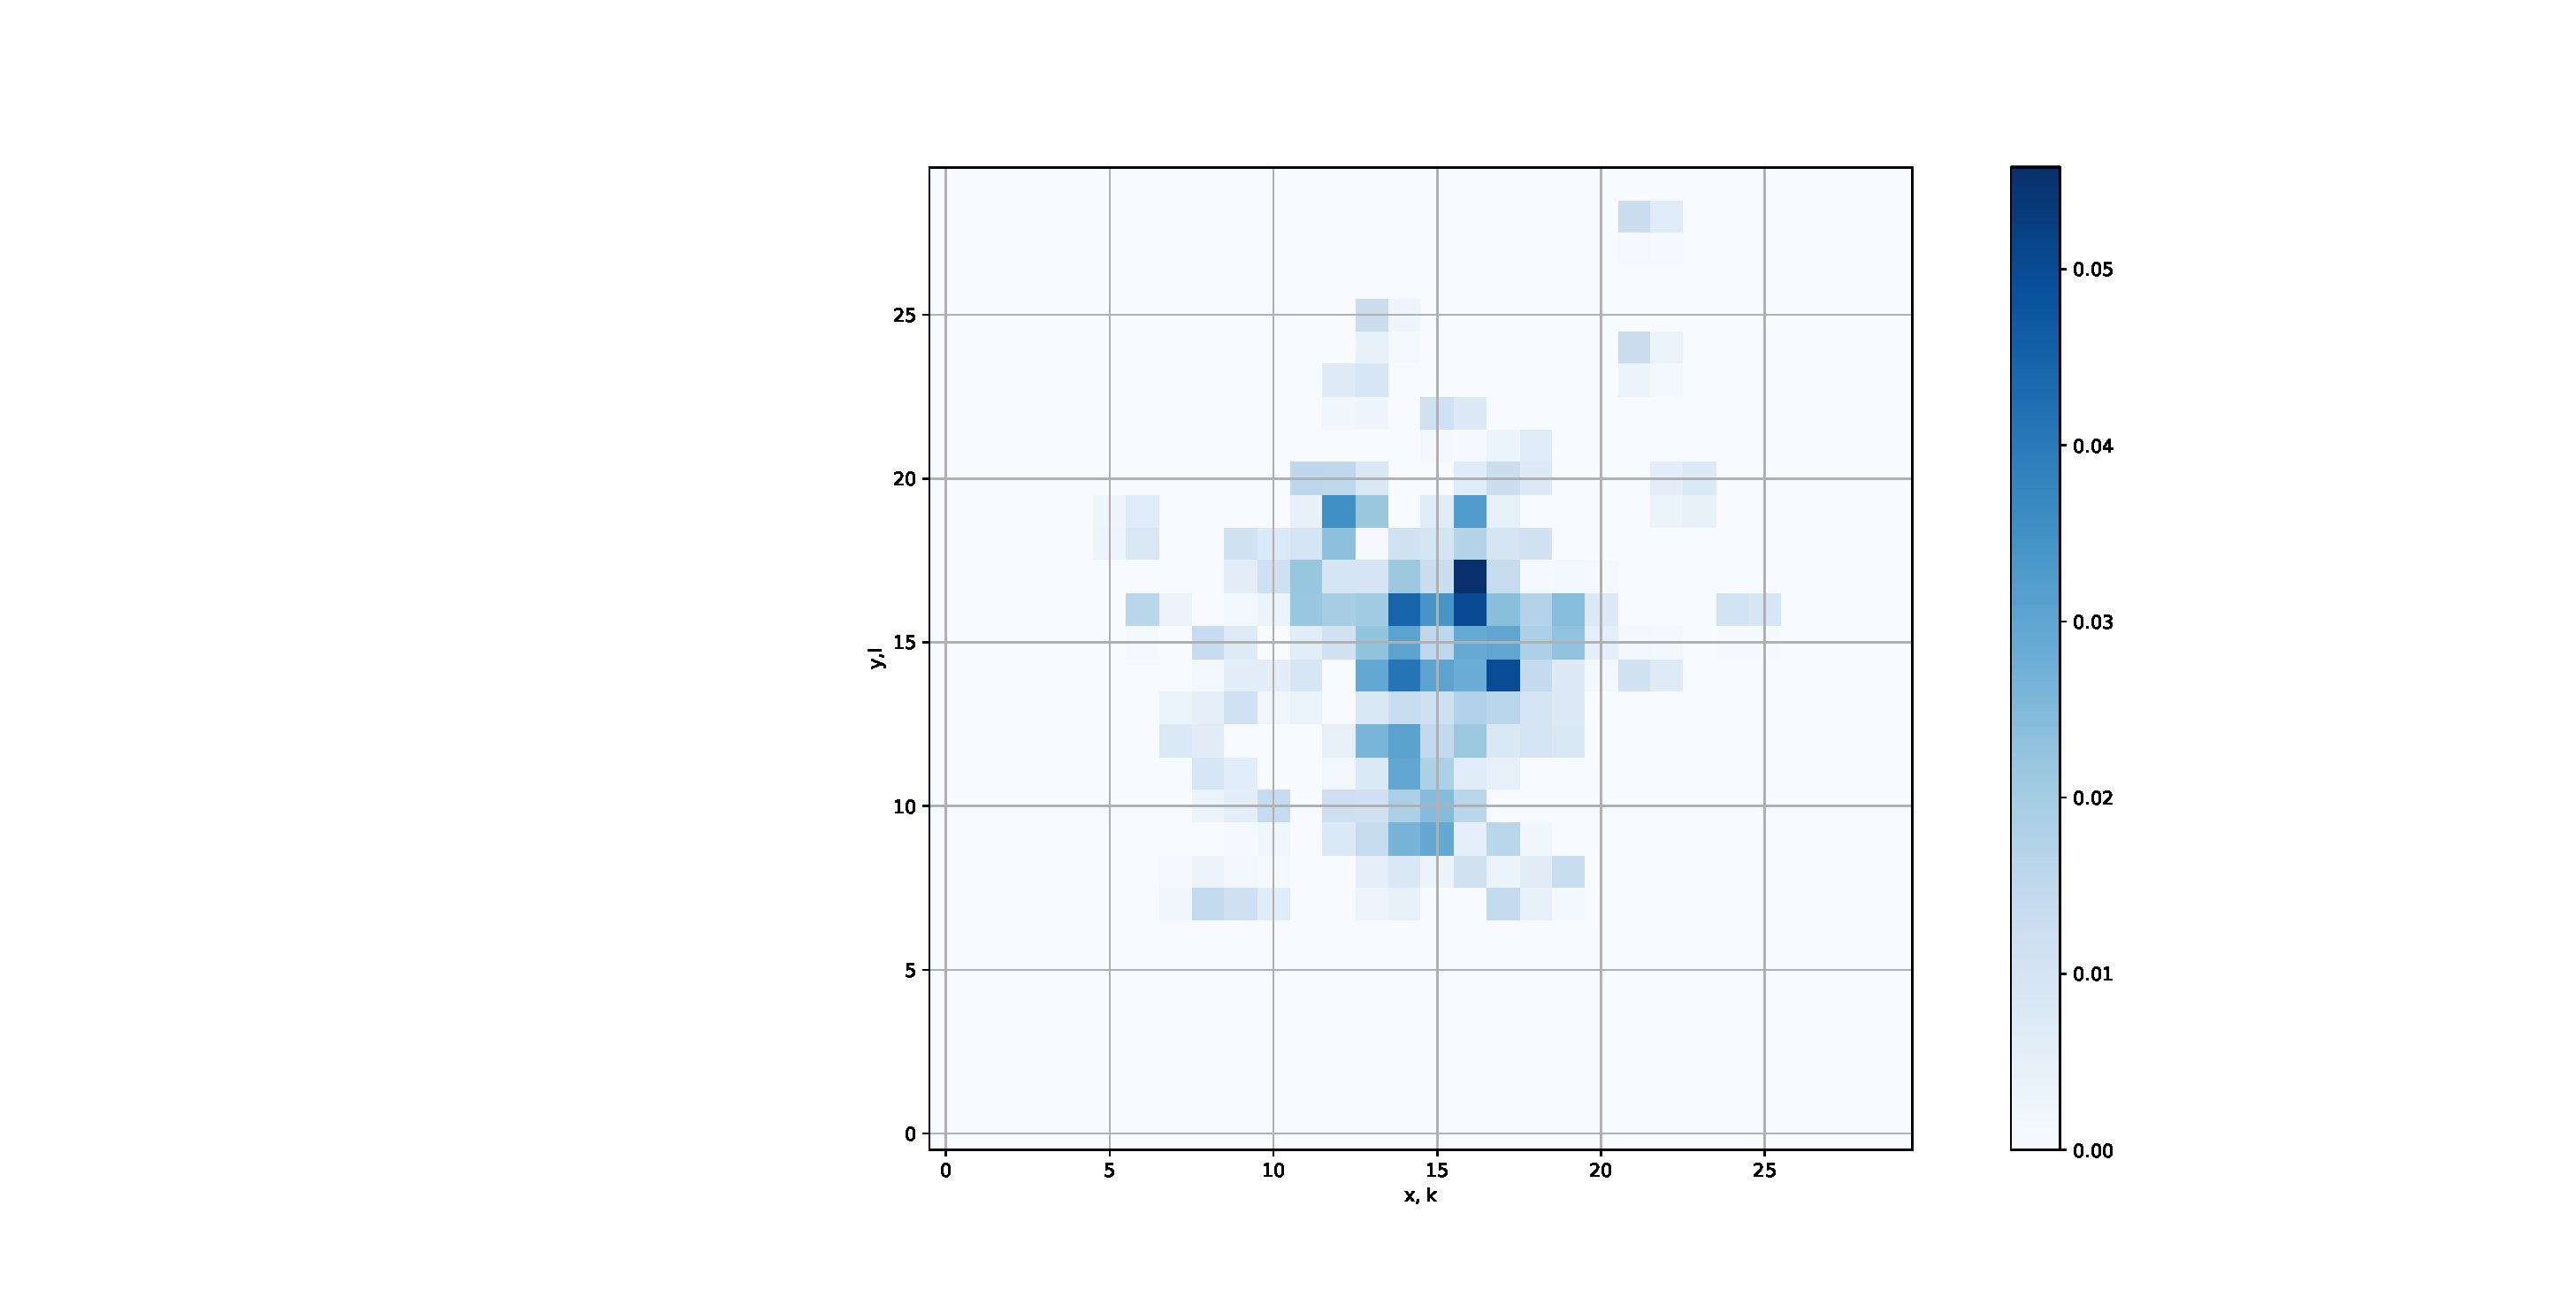
\includegraphics[width=0.9\linewidth]{Plots/N100_1}
	\caption{100 particles on the grid with the \(1^{st}\)-order method.}
	\label{fig:n1001}
\end{figure}
\begin{figure}[h]
	\centering
	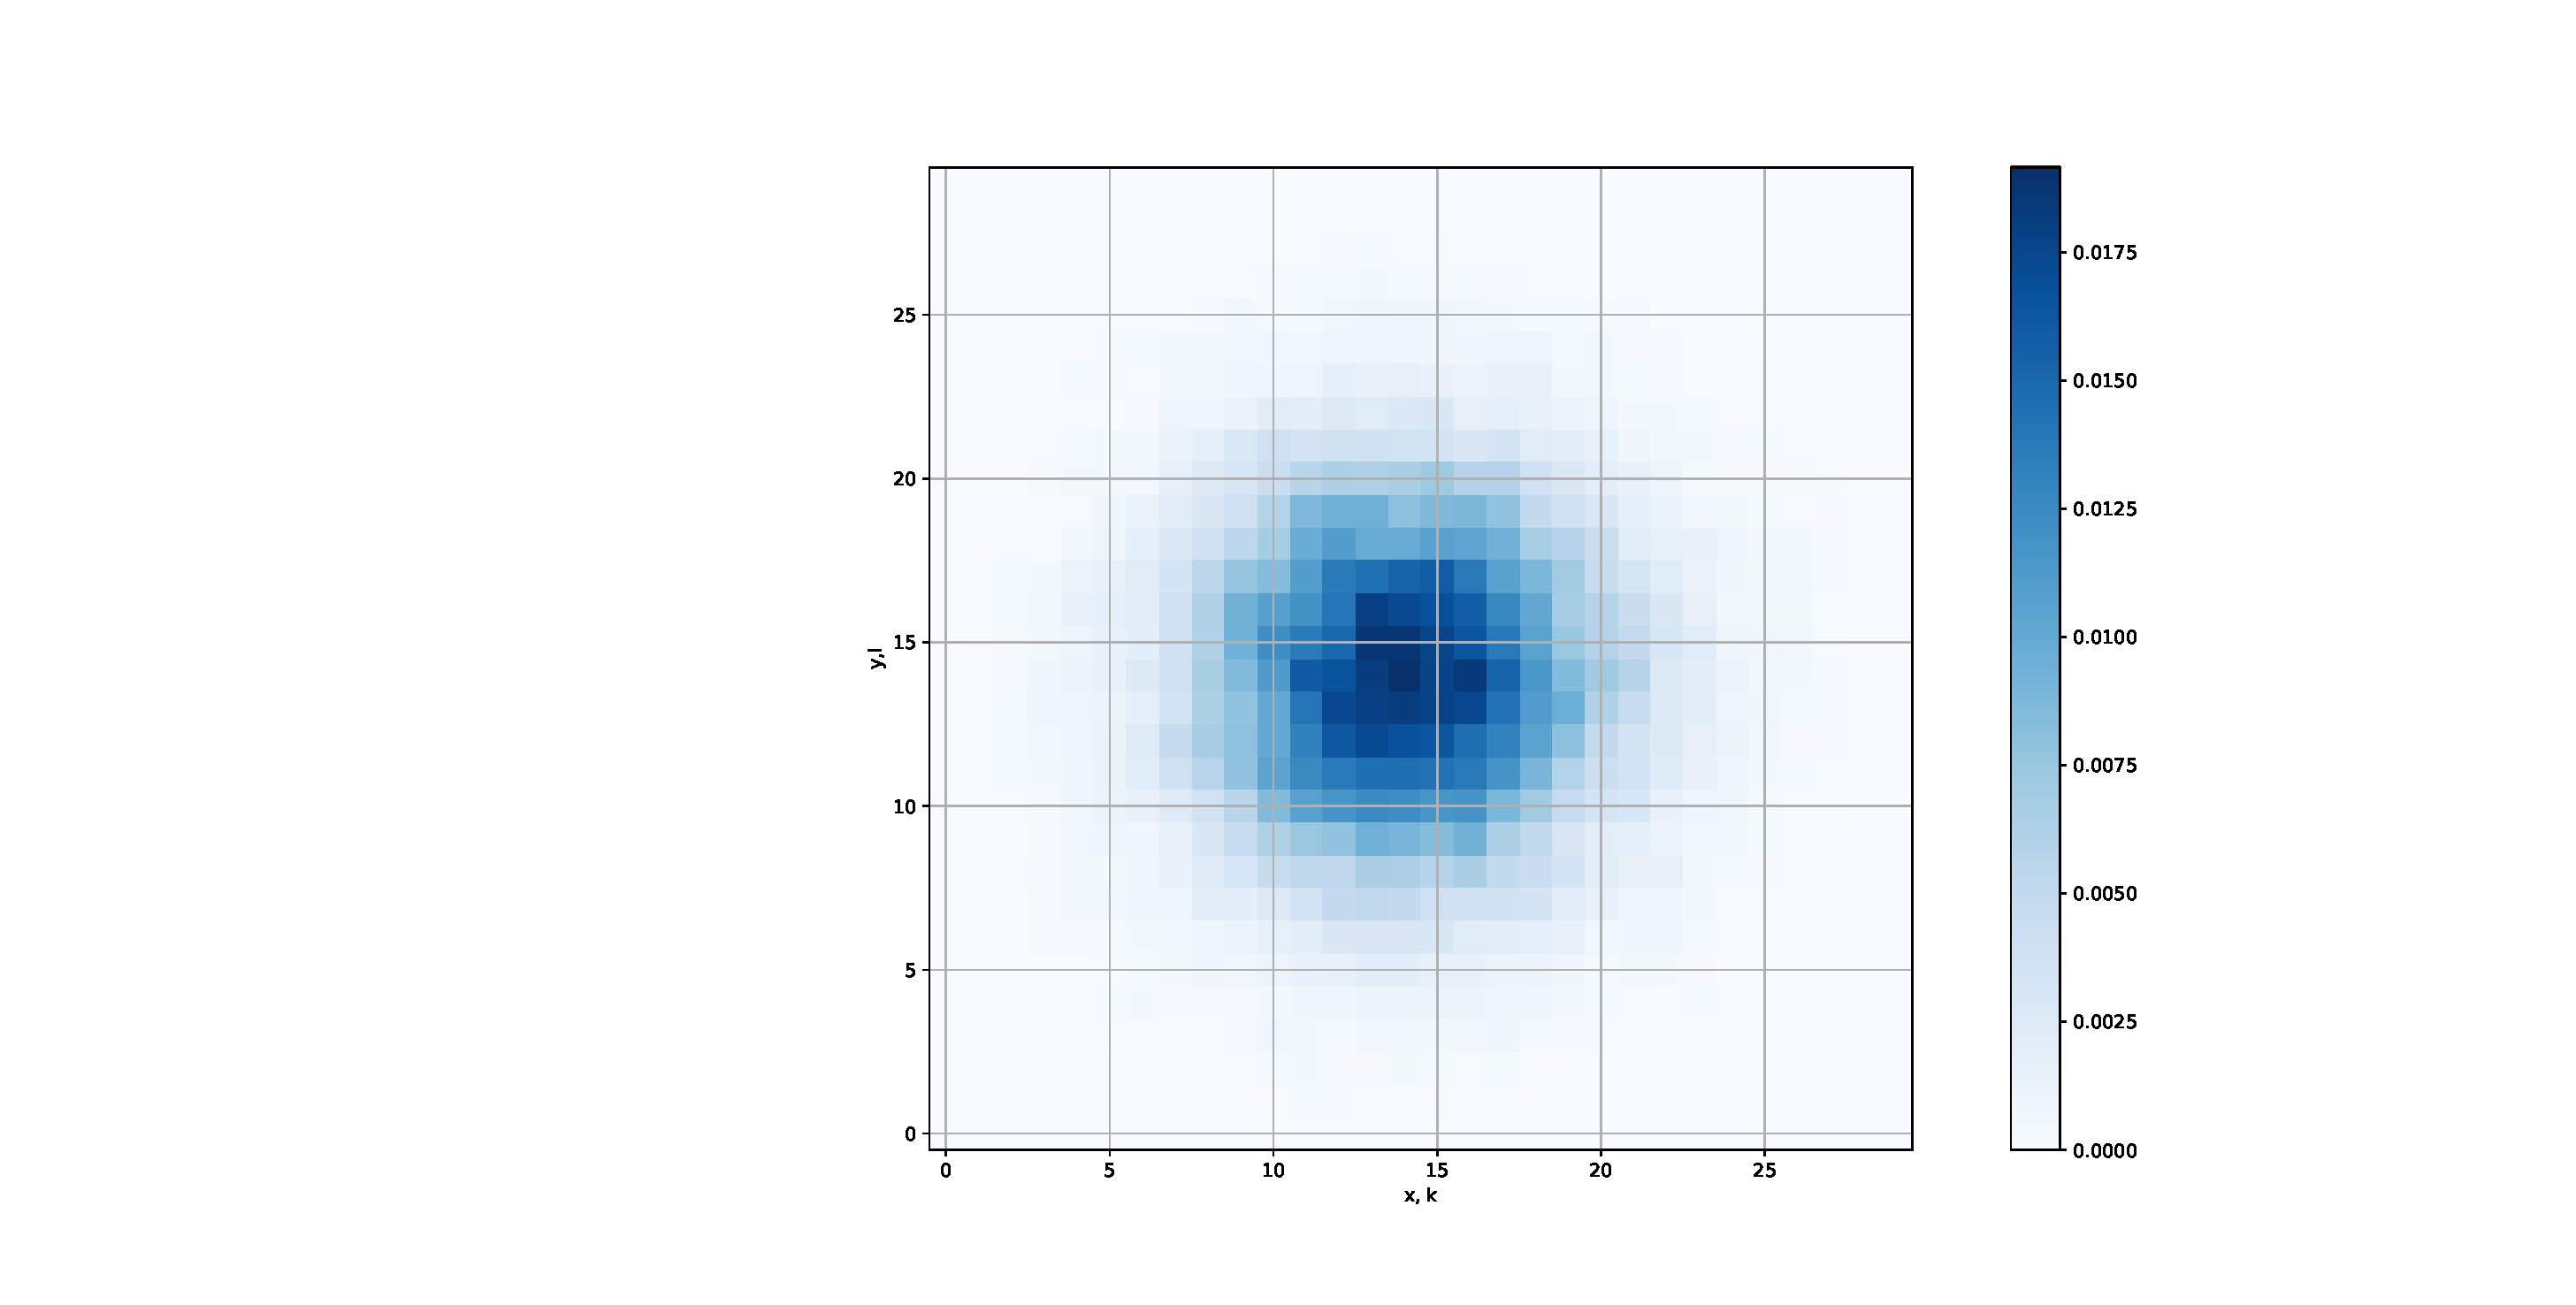
\includegraphics[width=0.9\linewidth]{Plots/N10000_2}
	\caption{100 particles on the grid with the \(2^{nd}\)-order method.}
	\label{fig:n1002}
\end{figure}\newpage
Lastly, we analyze the same for 10000 particles (figures \ref{fig:n100000}, \ref{fig:n100001} and \ref{fig:n100002}). When calculating the sum over the density matrix, we got the following results:
\begin{align}
	\sum_{kl} \rho_{kl}^0 \approx 1.985\\
	\sum_{kl} \rho_{kl}^1 \approx 1.996\\
	\sum_{kl} \rho_{kl}^2 \approx 1.998
\end{align}
This is in good agreement with expected value of \(2\).
\begin{figure}[h]
	\centering
	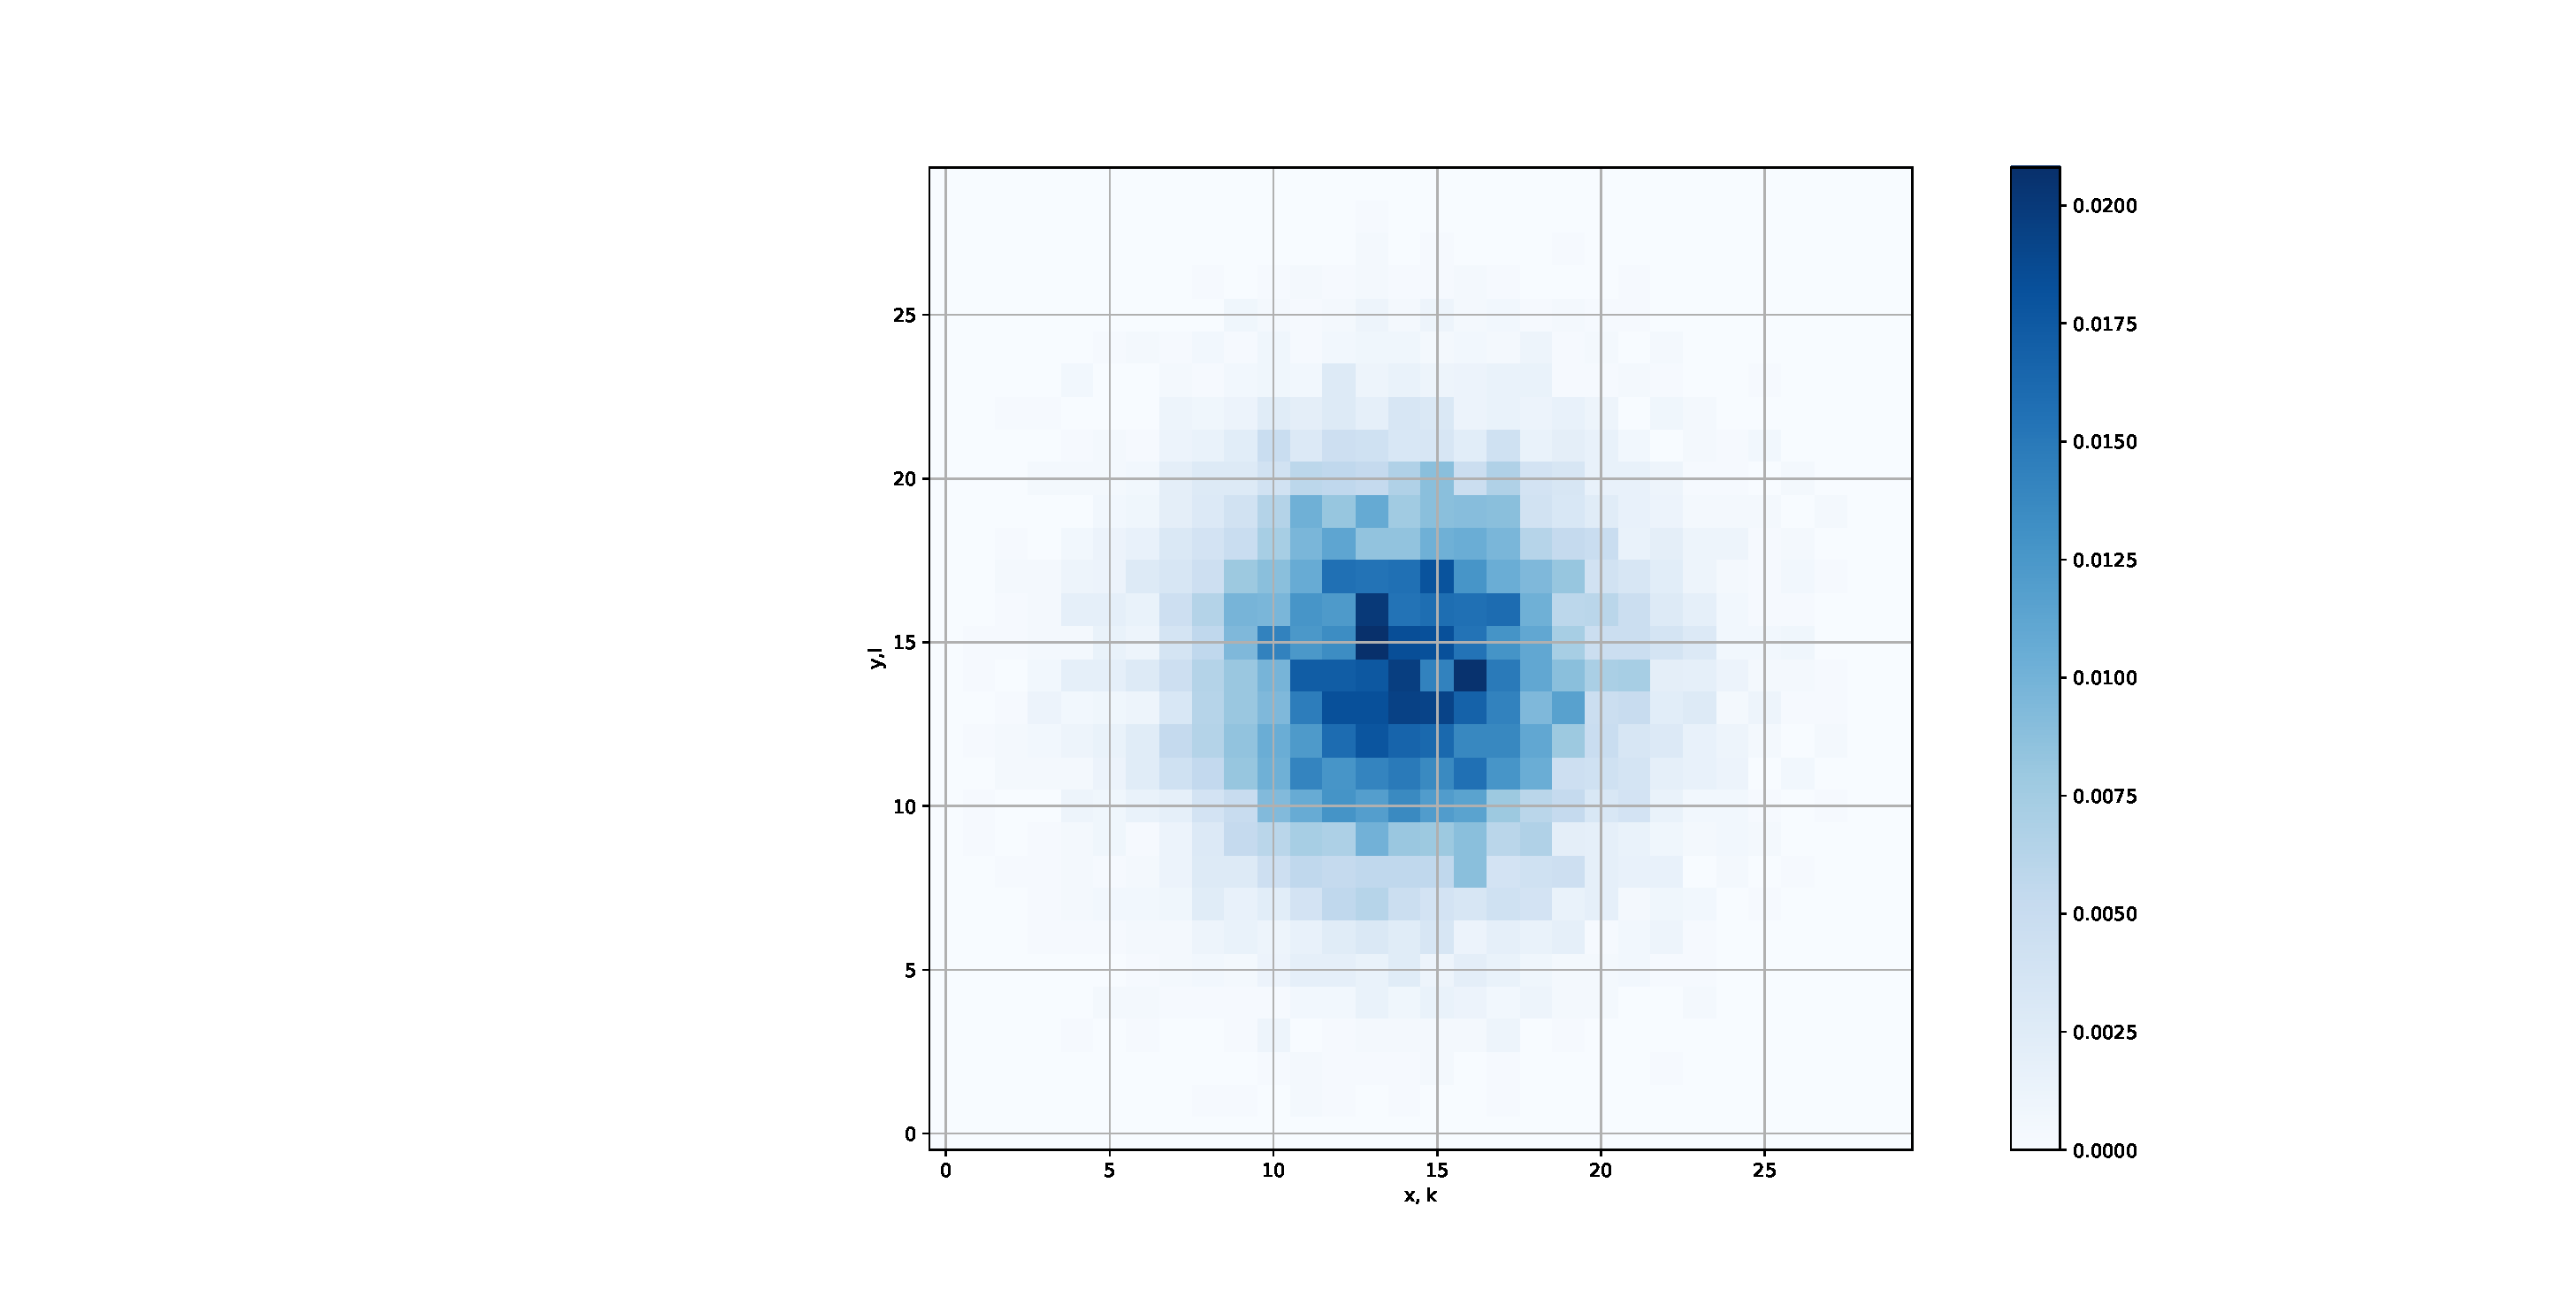
\includegraphics[width=0.9\linewidth]{Plots/N10000_0}
	\caption{10000 particles on the grid with the \(0^{th}\)-order method.}
	\label{fig:n100000}
\end{figure}
\begin{figure}[h]
	\centering
	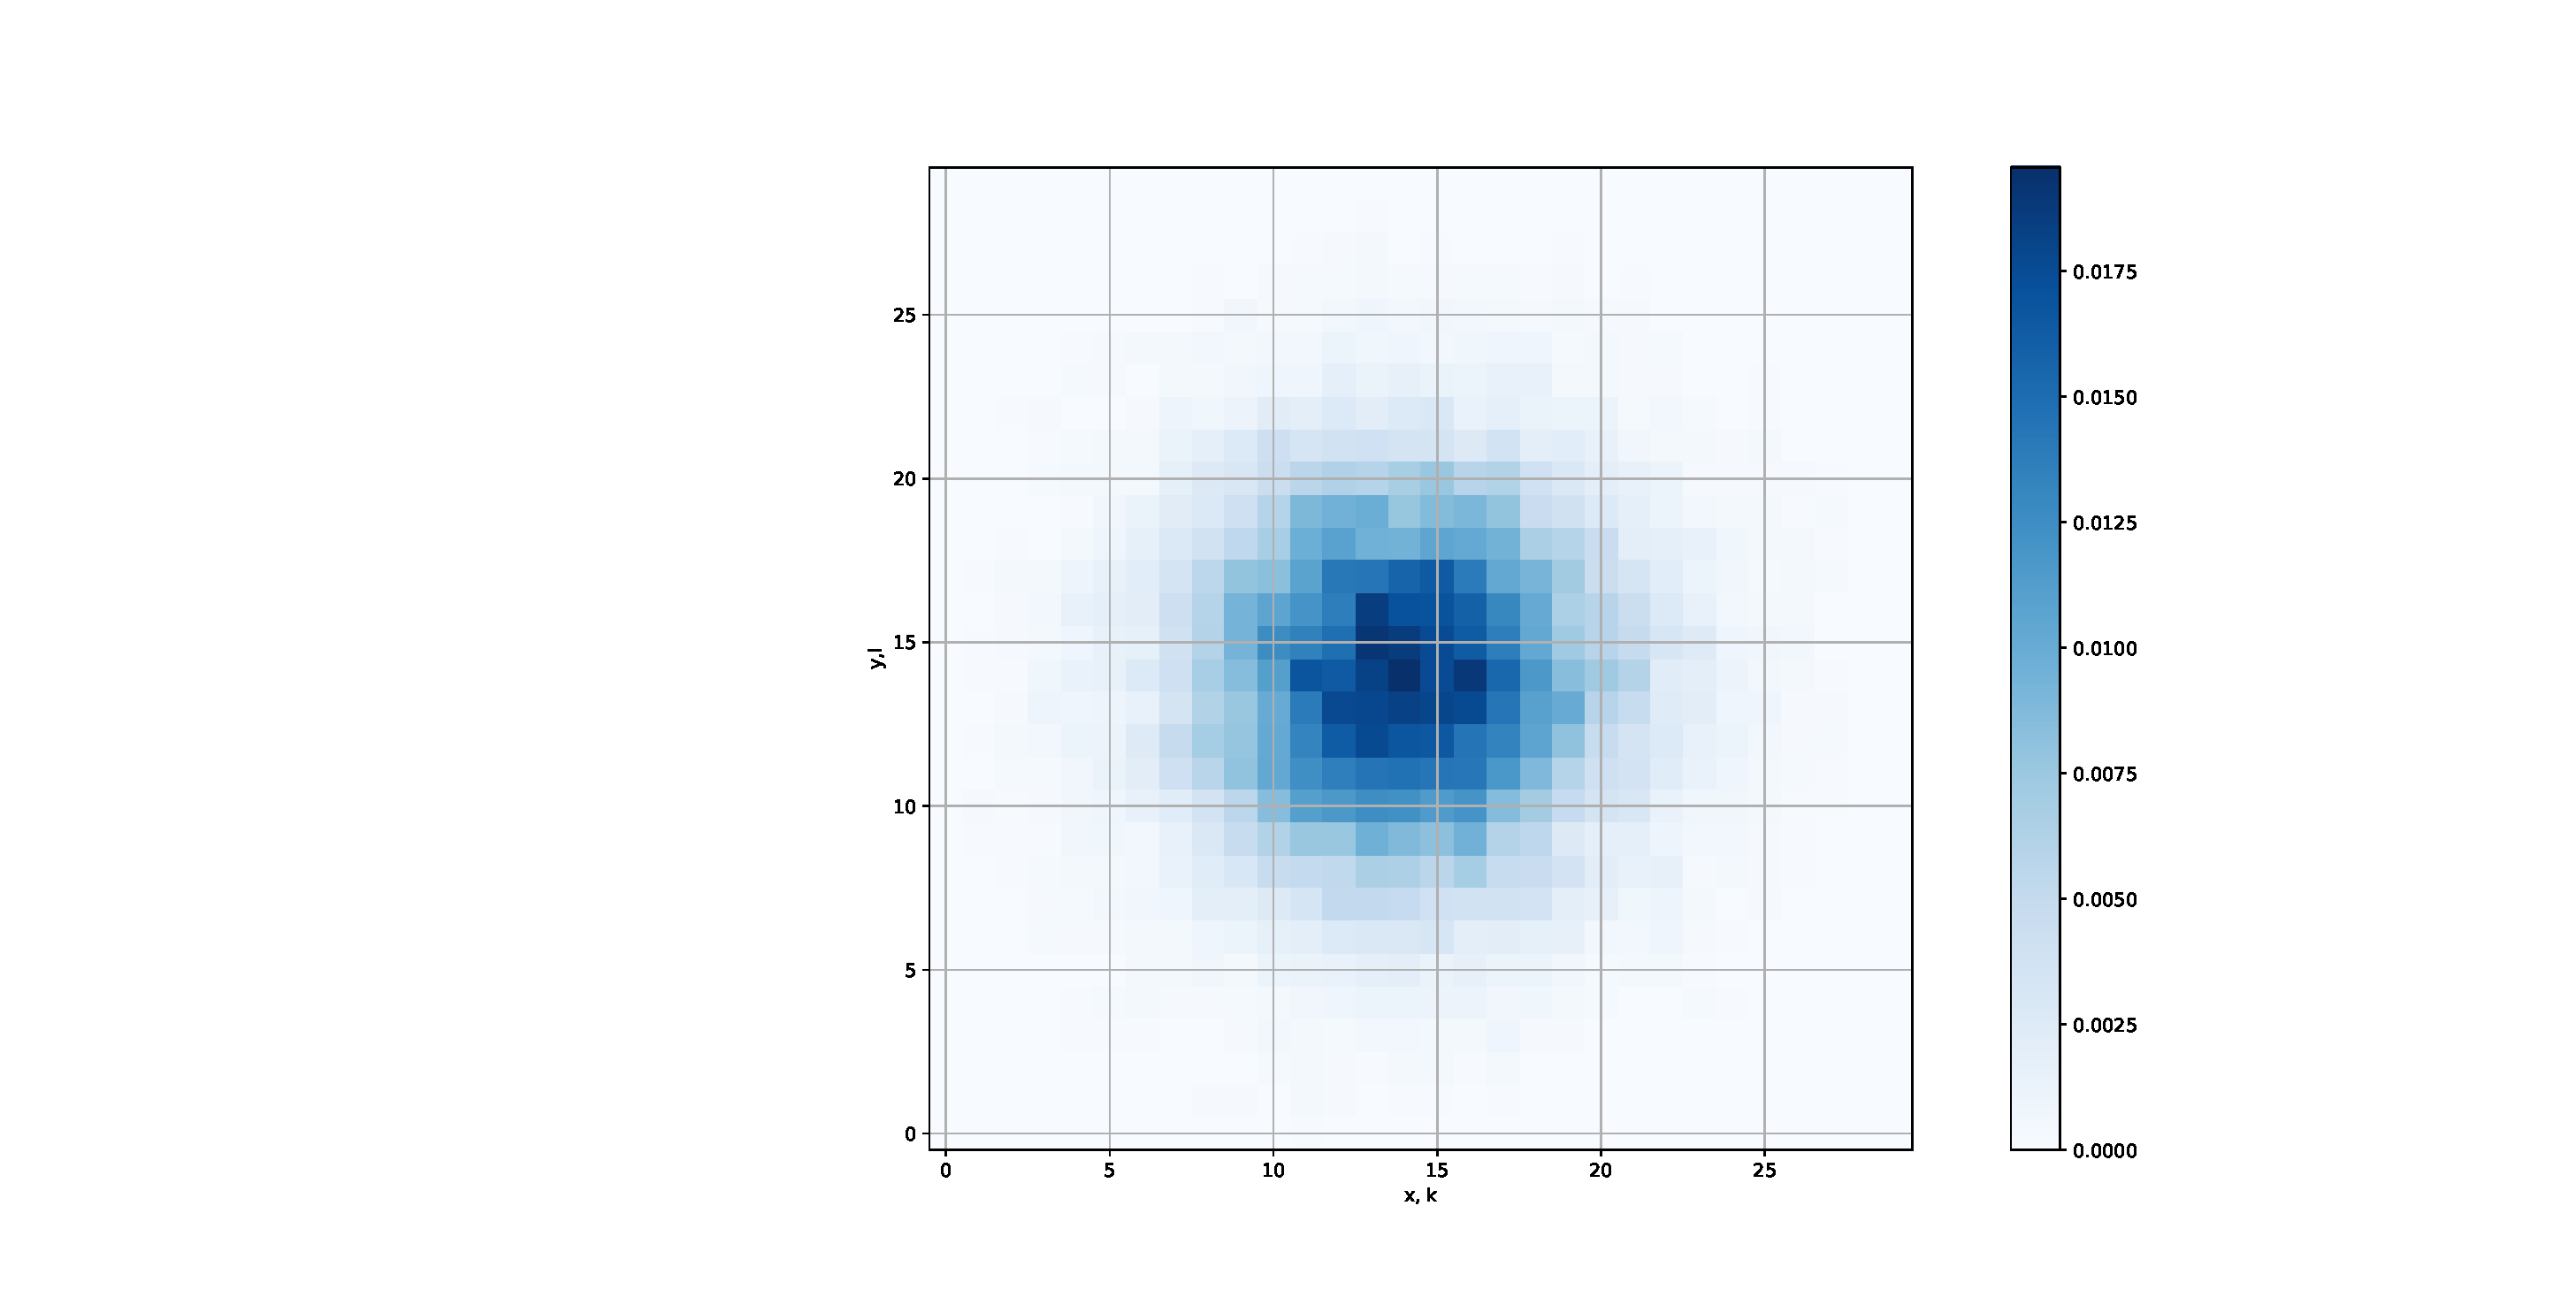
\includegraphics[width=0.9\linewidth]{Plots/N10000_1}
	\caption{10000 particles on the grid with the \(1^{st}\)-order method.}
	\label{fig:n100001}
\end{figure}
\begin{figure}[h]
	\centering
	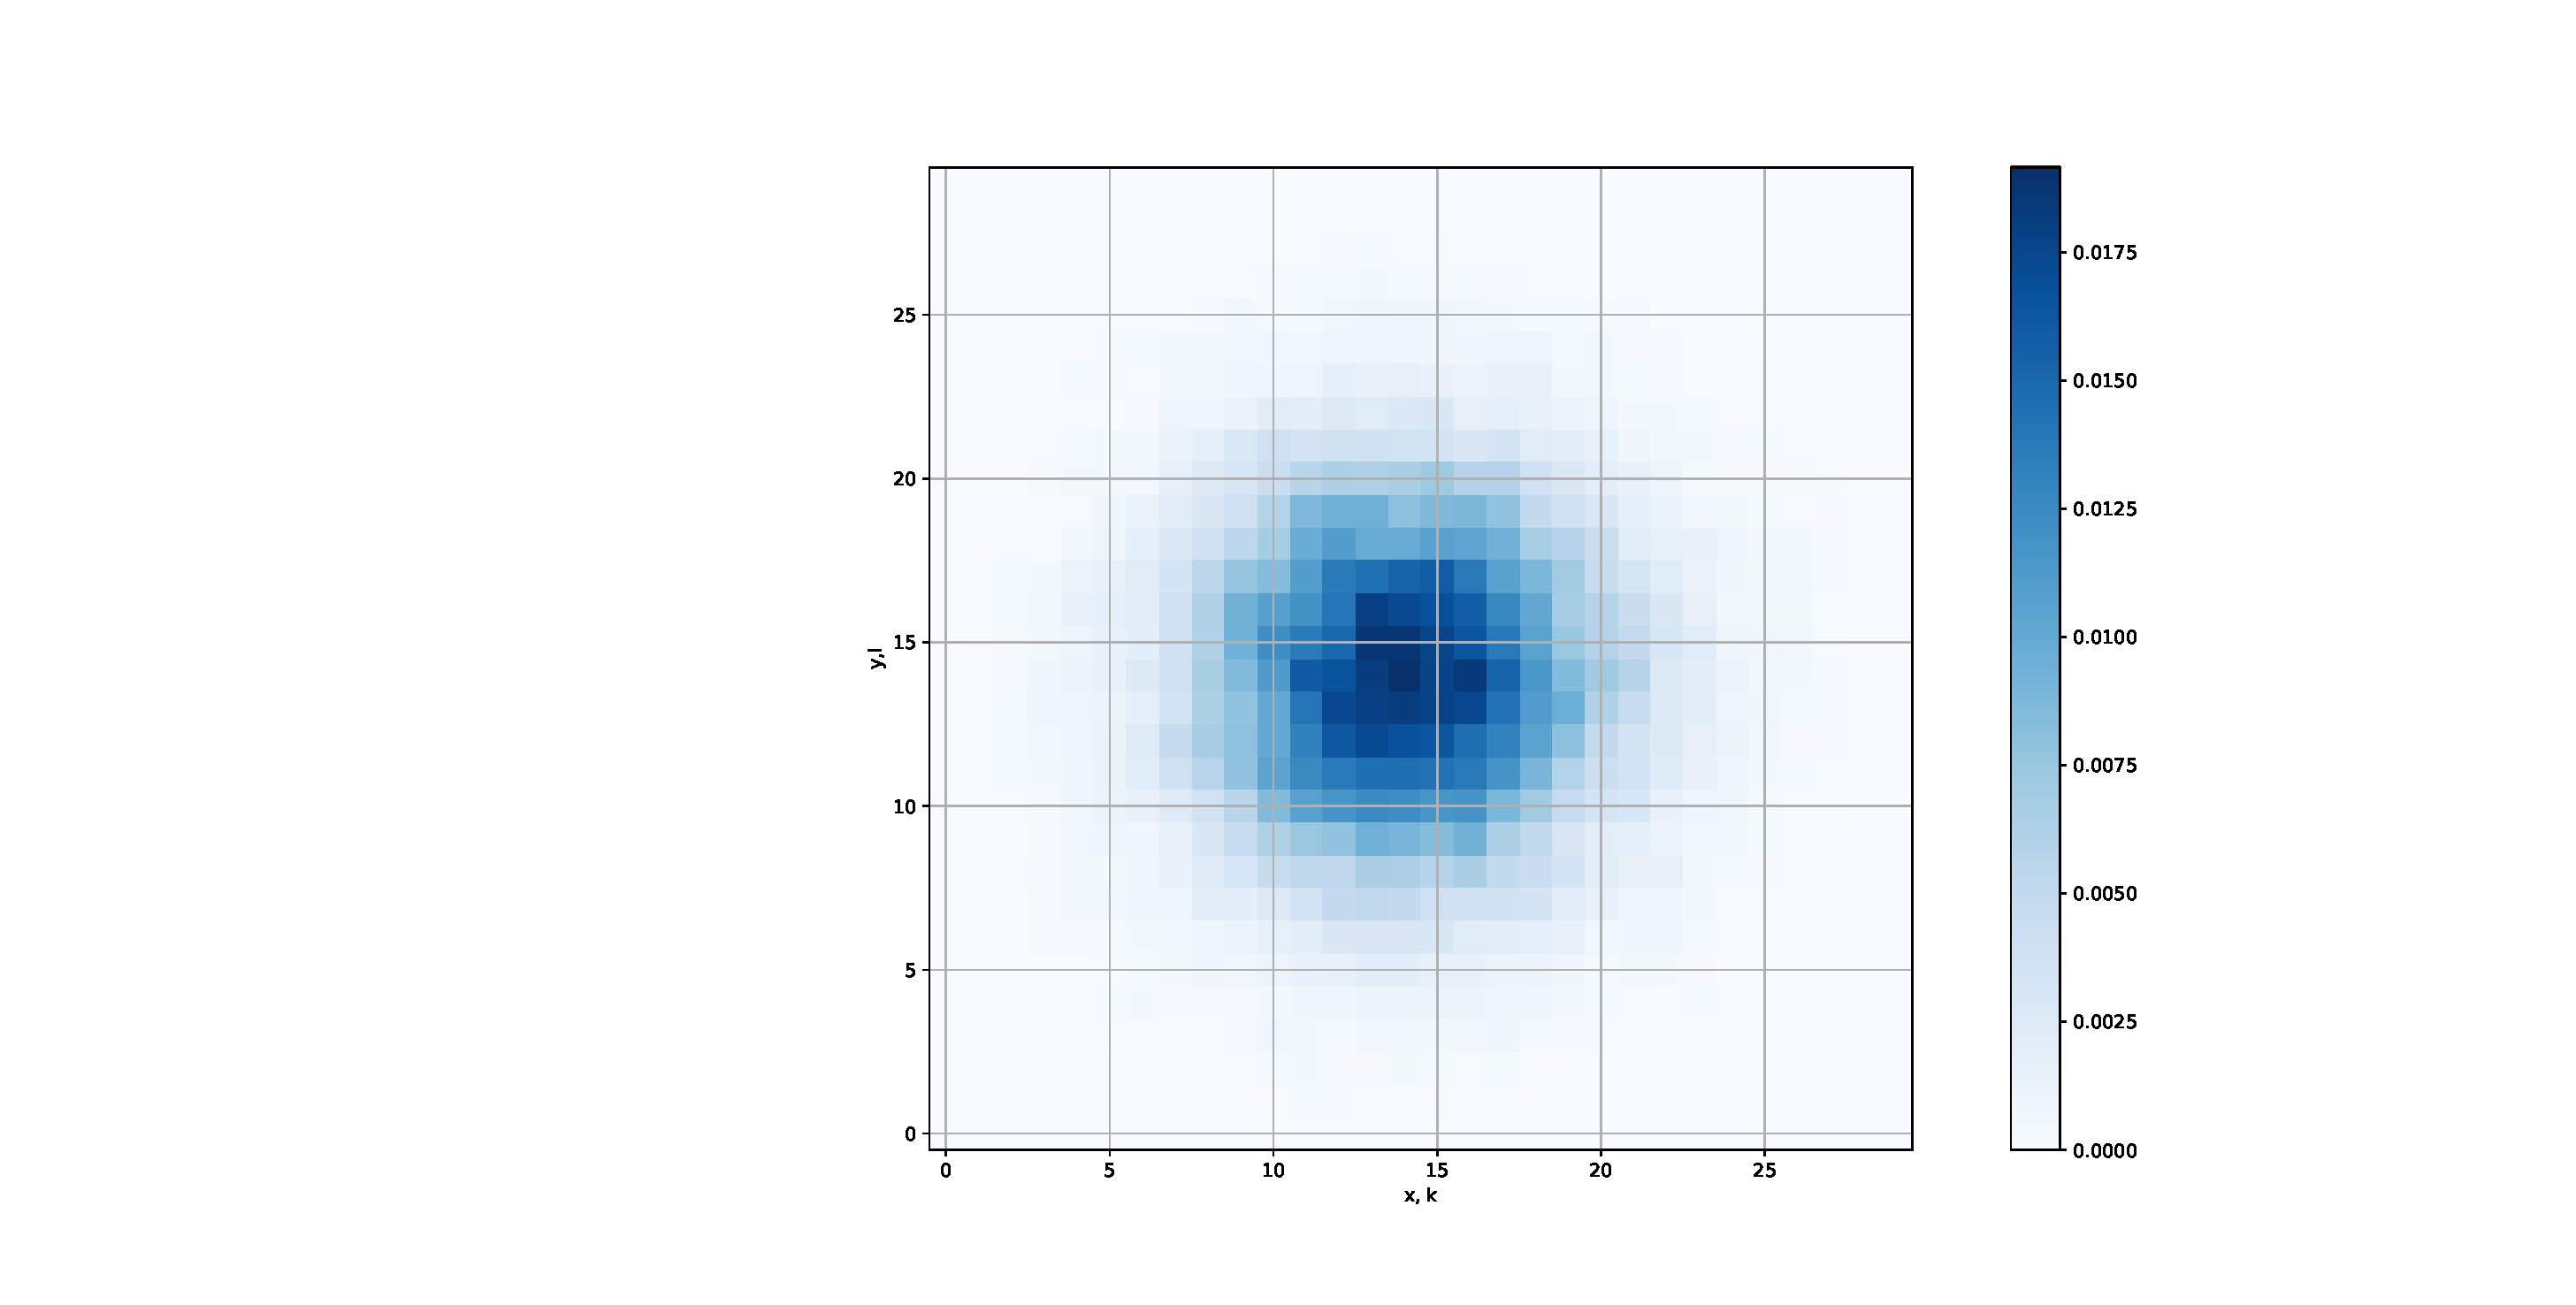
\includegraphics[width=0.9\linewidth]{Plots/N10000_2}
	\caption{10000 particles on the grid with the \(2^{nd}\)-order method.}
	\label{fig:n100002}
\end{figure}


\end{document}
